\documentclass[table]{beamer}
\usepackage{amsthm, amsmath, amssymb}
\usepackage[noplaybutton]{media9}
\usepackage{subfig}
\captionsetup[subfigure]{labelformat=empty}
\usepackage{tikz}
\usetikzlibrary{fadings}
\usetikzlibrary{arrows,shapes, positioning}
\usepackage{color}

\usepackage{centernot} % for negating symbols

\usepackage{multirow} % for tables with multi row spanning elements
\usepackage{booktabs}

\includeonlyframes{current,}

\tikzset{onslide/.code args={<#1>#2}{%
  \only<#1>{\pgfkeysalso{#2}} 
}}

% This is to patch the issue with missing unicode-data package. Still illusive but it works.
\usepackage{sansmathaccent}
\pdfmapfile{+sansmathaccent.map}

\usetheme{default}
\useinnertheme{rounded}
\usecolortheme{crane}

\definecolor{myblue}{rgb}{0.753,0.85,1}
\beamertemplatenavigationsymbolsempty

\setbeamercolor{normal text}{fg=white,bg=black}
\setbeamercolor{structure}{fg=white}

\setbeamercolor{alerted text}{fg=red!85!black}

\setbeamercolor{item projected}{use=item,fg=black,bg=myblue!60}

\setbeamercolor*{palette primary}{use=structure,fg=structure.fg}
\setbeamercolor*{palette secondary}{use=structure,fg=structure.fg!95!black}
\setbeamercolor*{palette tertiary}{use=structure,fg=structure.fg!90!black}
\setbeamercolor*{palette quaternary}{use=structure,fg=structure.fg!95!black,bg=black!80}
\setbeamercolor*{framesubtitle}{fg=black}

%\setbeamercolor*{block title}{parent=structure,bg=orange!85}
\setbeamercolor*{block title}{fg=black,bg=myblue!60}
\setbeamercolor*{block body}{fg=black,bg=myblue!10}
\setbeamercolor*{block title alerted}{parent=alerted text,bg=myblue!15}
\setbeamercolor*{block title example}{parent=example text,bg=myblue!15}
\setbeamercolor{frametitle}{fg=black,bg=myblue!60}
\setbeamercolor{title}{fg=black,bg=myblue!60}


% Below will make all title page transparent
%\addtobeamertemplate{title page bg}{\pgfsetfillopacity{0.5}}{\pgfsetfillopacity{1}}
%
% below will add logo on every frametitle banner, but needs new package. Whe you're all done with the slides, try to uninstall and reinstall miktex and cross fingers.
%\usepackage{textpos}
%\addtobeamertemplate{frametitle}{}{%
%\begin{textblock*}{10cm}(\textwidth,-1cm)
%
\includegraphics[height=1cm,width=1cm,keepaspectratio]{media/logo-sheffield-2.png}
%\end{textblock*}}

\title{Magneto-acoustic waves in an asymmetric magnetic slab}
\subtitle{Progress in spatial magneto-seismology}
\author{\hspace*{2.8in} \textbf{Matthew Allcock} \\ \hspace*{2.8in} \small and \\ \hspace*{2.8in}\vspace*{-1.4in} Robertus Erd\'{e}lyi}
%\date{\hspace*{2.8in}\vspace*{-1.6in}20th April 2017}
\date{}
\titlegraphic{\vspace*{0.9in}\hspace*{2.8in}
\includegraphics[height=1cm]{media/logo-sheffield-2.png}\hspace*{0.2in}
\includegraphics[height=1.2cm]{media/sp2rc_logo2.png}}

%----------------------------------------------------------------------

\AtBeginSection[]
{
   \begin{frame}
       \frametitle{Outline}
       \tableofcontents[currentsection]
   \end{frame}
}

\begin{document}

{
\setbeamercolor*{background canvas}{bg=black}
\setbeamertemplate{background}{%
  \vbox to \paperheight{\vfil\hbox to \paperwidth{\hfil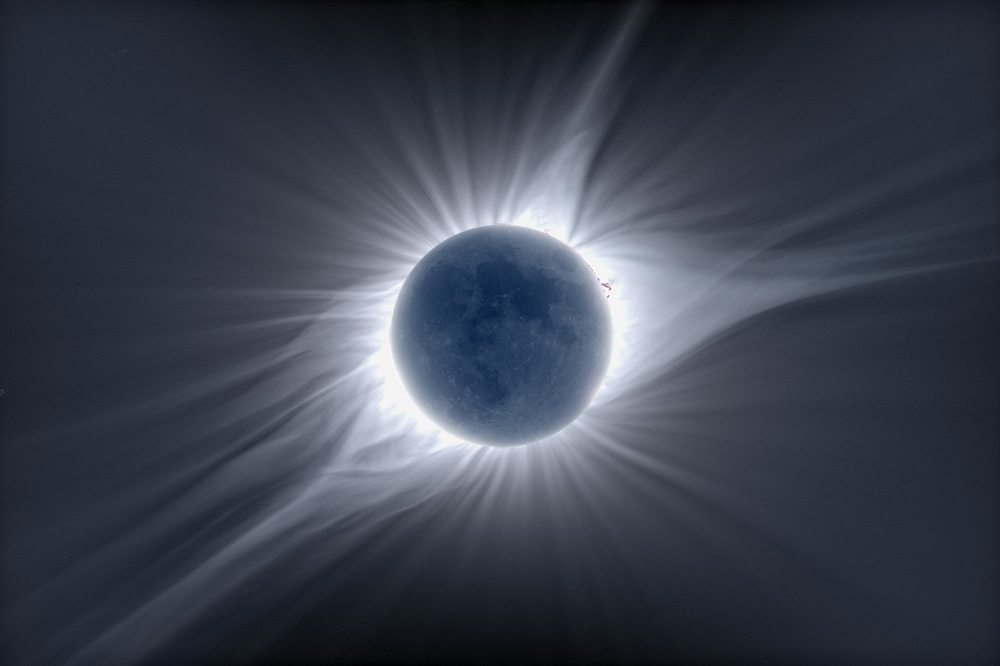
\includegraphics[width=\paperwidth]{{media/eclipse-corona-aug-2017.jpg}}\hfil}}
}
\begin{frame}
  	\titlepage
\end{frame}
}

\begin{frame}
	\frametitle{Outline}
   	\tableofcontents
\end{frame}


\section{Introduction}
\subsection{Waves on the Sun}

\begin{frame}
\frametitle{Waves on the Sun}
\begin{columns}
\begin{column}{0.5\textwidth}
    \begin{center}
	Global pressure modes (p-modes):
	\begin{itemize}
	\item Standing modes,
	\item Spherical harmonics with global Sun as cavity,
	\item Global and local \textbf{helioseismology} for inference of sub-surface flows, density, temperature.
	\end{itemize}
    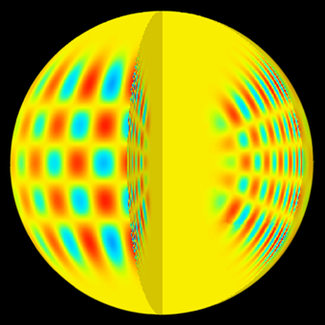
\includegraphics[width=0.6\textwidth]{media/helioseismology.png}
	\end{center}
\end{column}
\begin{column}{0.5\textwidth}
    \begin{center}
    MHD waves:
	\begin{itemize}
	\item Propagating or standing modes,
	\item Guided by local plasma inhomogeneity,
	\item Local \textbf{magneto-seismology} for inference of background magnetic field strength, heat transport coefficients, density.
	\end{itemize}
	\includemedia[
	  width=0.9\textwidth,
	  transparent,
	  addresource=media/coronal_loop_oscillations.mp4,
	  flashvars={
	  	source=media/coronal_loop_oscillations.mp4
	  	&loop=true
  	  }
	]{\centering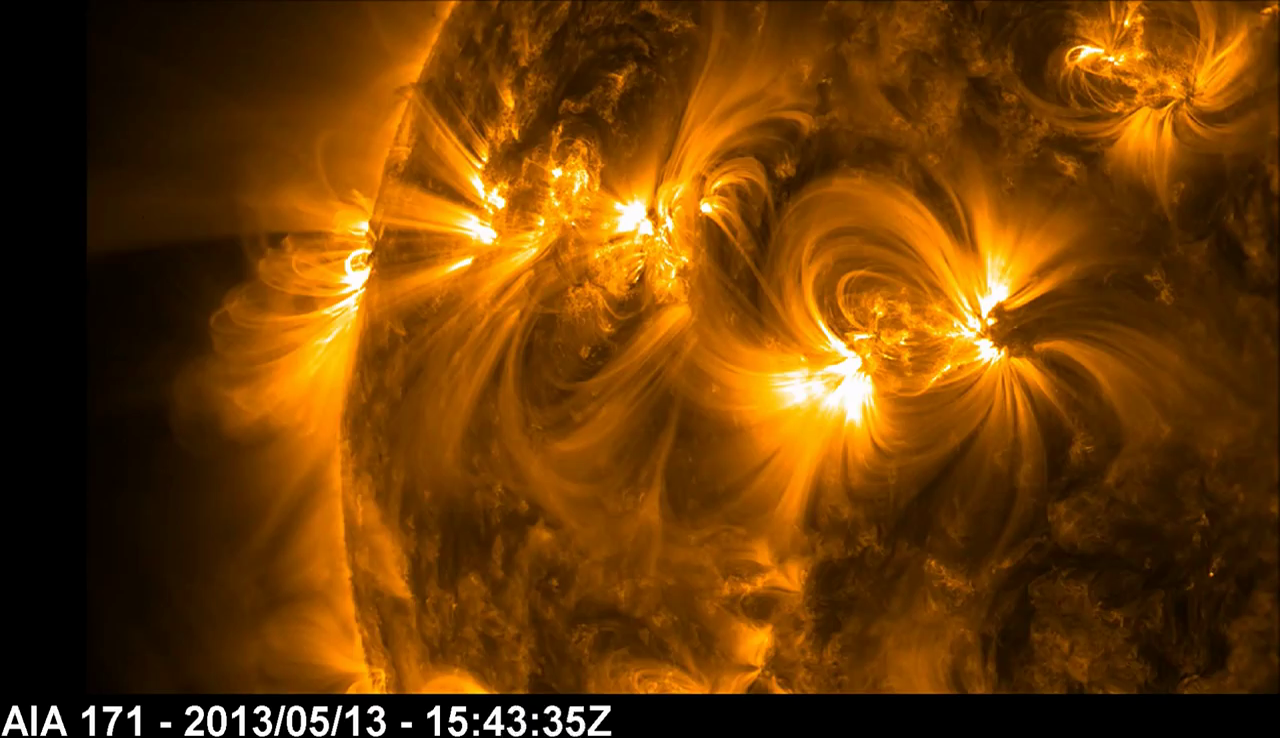
\includegraphics{media/coronal_loop_oscillations.png}}{VPlayer.swf}
	\end{center}
\end{column}
\end{columns}
\end{frame}

\subsection{Solar magneto-seismology (SMS)}

\begin{frame}
\frametitle{Solar magneto-seismology}
\framesubtitle{An overview}
%
%\color{black}
\newcommand{\tb}{\textcolor{black}}
\tikzstyle{format} = [draw, rounded corners=.055cm, fill=myblue!80]
\tikzstyle{medium} = [ellipse, draw, thin, fill=green!20, minimum height=2.5em]

\begin{figure}
\begin{tikzpicture}[node distance=1.8cm and 3.cm, auto, >=latex, align = flush center, ultra thick, on grid=true, font=\small]
    % We need to set at bounding box first. Otherwise the diagram
    % will change position for each frame.
    \path[use as bounding box] (-1,0) rectangle (10,-2);
    \path[onslide=<1>{alert}]<1-> node[format] (obs) {
    		\tb{Observations}};
    \path[]<1-> node[below= of obs] (ghost) {};
    \path[onslide=<4>{alert}]<4-> node[format, below= of ghost] (phys) {
    		\tb{Physical} \\ 
    		\tb{understanding}};
    		
    \path[onslide={<2,8>{alert}}, onslide=<10>{green}]<2-> node[format, below right= of obs] (ep) {
    		\tb{Equilibrium} \\ 
    		\tb{parameters}};
    \path[onslide=<2>{alert}]<2-> (ep) edge[<-] (obs);
    \path[onslide=<2>{alert}]<2-> node[format, above right= of obs] (wp) {
    		\tb{Wave} \\ 
    		\tb{parameters}}
    		edge[<-] (obs);
    		
    \path[onslide=<3>{alert}]<3-> node[format, right= of wp] (tp) {
    		\tb{Temporal} \\ 
    		\tb{parameters}}
    		edge[<-] (wp);
    \path[onslide=<3>{alert}]<3-> node[format, below= of tp] (sp) {
    		\tb{Spatial} \\ 
    		\tb{parameters}}
    		edge[<-] (wp)
    		edge[<-] (ep);  

    \path[onslide=<5>{alert}, onslide=<10>{green}]<5-> node[format, right= of phys] (em) {
    					\tb{Equilibrium} \\ 
    					\tb{models}};
    \path[onslide=<5>{alert}]<5-> (em) edge[<-] (phys);
                   
    \path[onslide=<6>{alert}, onslide=<10>{green}]<6-> node[format, right= of em] (eig) {
    					\tb{Eigenmodes}}
                   edge[<-] (em);
                   
    \path[onslide=<7>{alert}]<7-> node[format, right= of sp] (ts) {
    					\tb{Temporal} \\
    					\tb{magneto-seismology}};
    \path[onslide=<7>{alert}]<7-> (ts) edge[<-] (tp);
    \node <7-> at (6,-2) (ghost2) {};
    \draw <7-> [->, onslide=<7>{alert}] (ghost2.center) -- (ts);
    \draw <7-> [onslide=<7>{alert}] (ghost2.center) -- (eig);
    \path[onslide=<7>{alert}, onslide=<10>{green}]<7-> node[format, below right= of sp] (ss) {
    					\tb{Spatial} \\
    					\tb{magneto-seismology}};
    \draw <7-> [->, onslide=<7>{alert}, onslide=<10>{green}] (eig) -- (ss);
    \path[onslide=<7>{alert}]<7-> (ss) edge[<-] (sp);

    
    \path[onslide=<8>{alert}]<8-> (ts) edge[->] (ep);
	\path[onslide=<8>{alert}, onslide=<10>{green}]<8-> (ss) edge[->] (ep);
                 
\end{tikzpicture}
\end{figure}
\end{frame}


\subsection{A brief history}

\begin{frame}[label=current]
\frametitle{Solar magneto-seismology}
\framesubtitle{A brief history - \textcolor{yellow}{temporal} and \textcolor{cyan}{spatial} seismology}
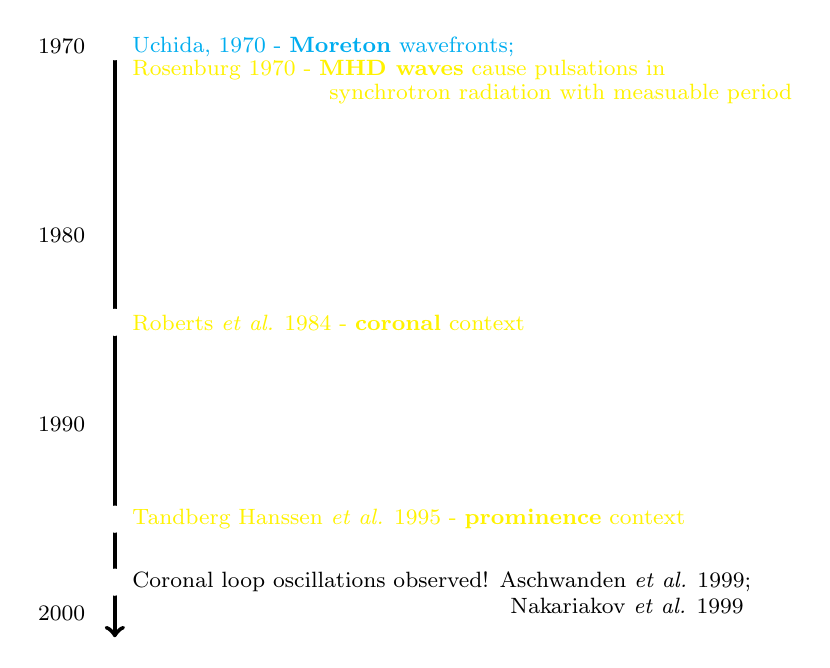
\begin{tikzpicture}[datemarker/.style={circle,draw=white,fill=white,radius=2pt}, 
textlabel/.style={anchor=west, font=\footnotesize}, temp/.style={color=yellow}, spat/.style={color=cyan}] 
\draw [<-, ultra thick] (0,-0.5) -- (0,7);
\draw (-1.1, 7) node [textlabel] {1970};
\draw (-1.1, 4.6) node [textlabel] {1980};
\draw (-1.1, 2.2) node [textlabel] {1990};
\draw (-1.1, -0.2) node [textlabel] {2000};
\pause

\node at (0, 7) [datemarker] {}; 
\draw (0.1, 7) node [textlabel, spat] {Uchida, 1970 - \textbf{Moreton} wavefronts;};
\pause
\draw (0.1, 6.7) node [textlabel, temp] {Rosenburg 1970 - \textbf{MHD waves} cause pulsations in};
\draw (2.6, 6.4) node [textlabel, temp] {synchrotron radiation with measuable period}; 
\pause
\node at (0, 3.5) [datemarker] {}; 
\draw (0.1, 3.5) node [textlabel, temp] {Roberts \textit{et al.} 1984 - \textbf{coronal} context};
\pause
\node at (0, 1.) [datemarker] {}; 
\draw (0.1, 1.) node [textlabel, temp] {Tandberg Hanssen \textit{et al.} 1995 - \textbf{prominence} context};
\pause
\node at (0, 0.2) [datemarker] {}; 
\draw (0.1, 0.2) node [textlabel] {Coronal loop oscillations observed! Aschwanden \textit{et al.} 1999;};
\draw (4.9, -0.1) node [textlabel] {Nakariakov \textit{et al.} 1999};
\end{tikzpicture}
\end{frame}


\begin{frame}[label=current]
\frametitle{Solar magneto-seismology}
\framesubtitle{A brief history - \textcolor{yellow}{temporal} and \textcolor{cyan}{spatial} seismology}
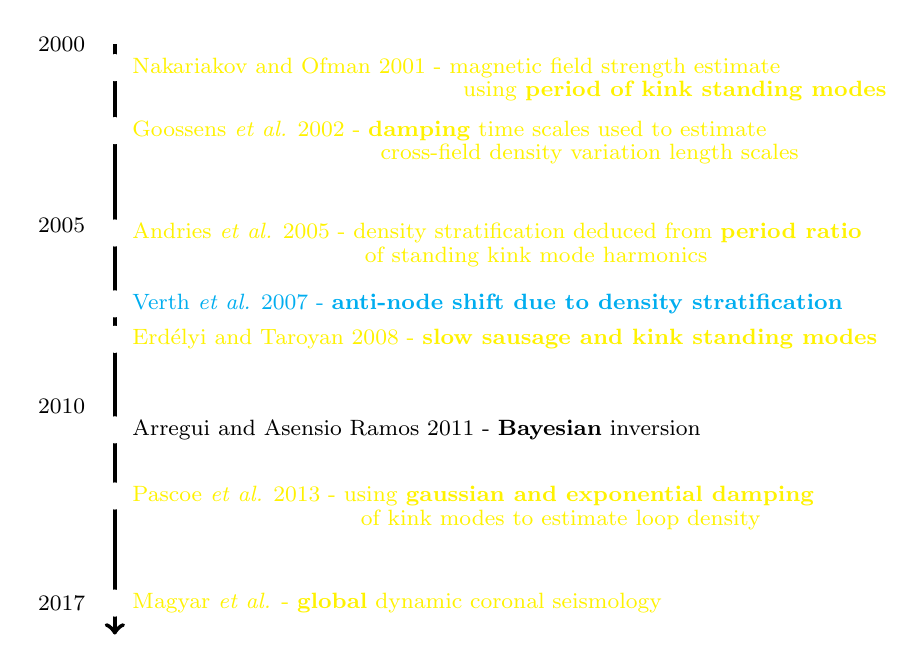
\begin{tikzpicture}[datemarker/.style={circle,draw=white,fill=white,radius=2pt}, 
textlabel/.style={anchor=west, font=\footnotesize}, temp/.style={color=yellow}, spat/.style={color=cyan}]
\draw [<-, ultra thick] (0,-0.5) -- (0,7);
\draw (-1.1, 7) node [textlabel] {2000};
\draw (-1.1, 4.7) node [textlabel] {2005};
\draw (-1.1, 2.4) node [textlabel] {2010};
\draw (-1.1, -0.1) node [textlabel] {2017};
\pause

\node at (0, 6.7) [datemarker] {}; 
\draw (0.1, 6.7) node [textlabel, temp] {Nakariakov and Ofman 2001 - magnetic field strength estimate};
\draw (4.3, 6.4) node [textlabel, temp] {using \textbf{period of kink standing modes}};
\pause
 
\node at (0, 5.9) [datemarker] {}; 
\draw (0.1, 5.9) node [textlabel, temp] {Goossens \textit{et al.} 2002 - \textbf{damping} time scales used to estimate};
\draw (3.25, 5.6) node [textlabel, temp] {cross-field density variation length scales};
\pause

\node at (0, 4.6) [datemarker] {}; 
\draw (0.1, 4.6) node [textlabel, temp] {Andries \textit{et al.} 2005 - density stratification deduced from \textbf{period ratio}};
\draw (3.05, 4.3) node [textlabel, temp] {of standing kink mode harmonics};
\pause

\node at (0, 3.7) [datemarker] {}; 
\draw (0.1, 3.7) node [textlabel, spat] {Verth \textit{et al.} 2007 - \textbf{anti-node shift due to density stratification}};
\pause
\node at (0, 3.25) [datemarker] {}; 
\draw (0.1, 3.25) node [textlabel, temp] {Erd\'{e}lyi and Taroyan 2008 - \textbf{slow sausage and kink standing modes}}; 
\pause
\node at (0, 2.1) [datemarker] {}; 
\draw (0.1, 2.1) node [textlabel] {Arregui and Asensio Ramos 2011 - \textbf{Bayesian} inversion};
\pause
\node at (0, 1.26) [datemarker] {}; 
\draw (0.1, 1.26) node [textlabel, temp] {Pascoe \textit{et al.} 2013 - using \textbf{gaussian and exponential damping}};
\draw (3, 0.96) node [textlabel, temp] {of kink modes to estimate loop density};
\pause
\node at (0, -0.1) [datemarker] {}; 
\draw (0.1, -0.1) node [textlabel, temp] {Magyar \textit{et al.} - \textbf{global} dynamic coronal seismology};
\end{tikzpicture}
\end{frame}


\section{SMS with asymmetric wave-guides}
\subsection{Motivation}

\begin{frame}
\frametitle{Asymmetric magnetic slab}
\framesubtitle{Motivation}
\centering
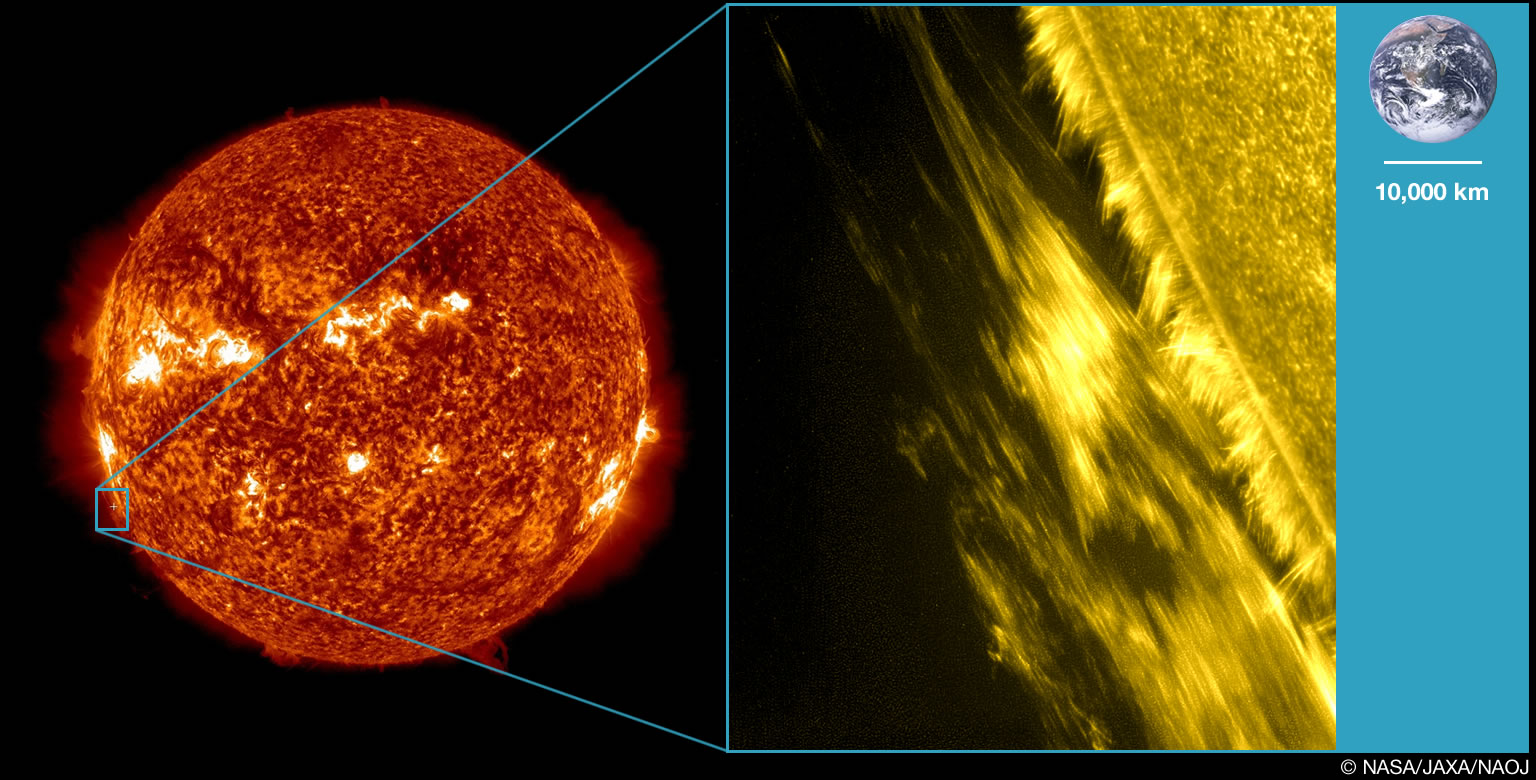
\includegraphics[height=4.5cm]{media/hinode-prominence.jpg}
\\
\vspace*{0.05in}
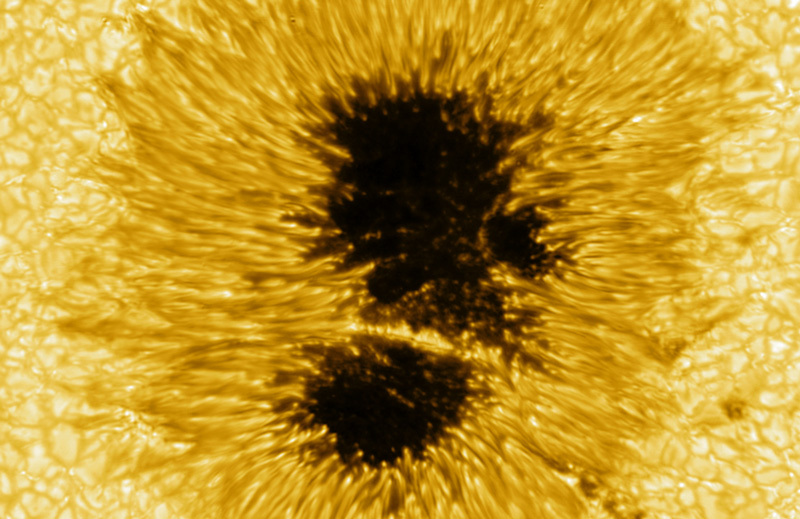
\includegraphics[height=3.5 cm]{media/sunspot_lightbridge.png}
\hspace*{0.5in}
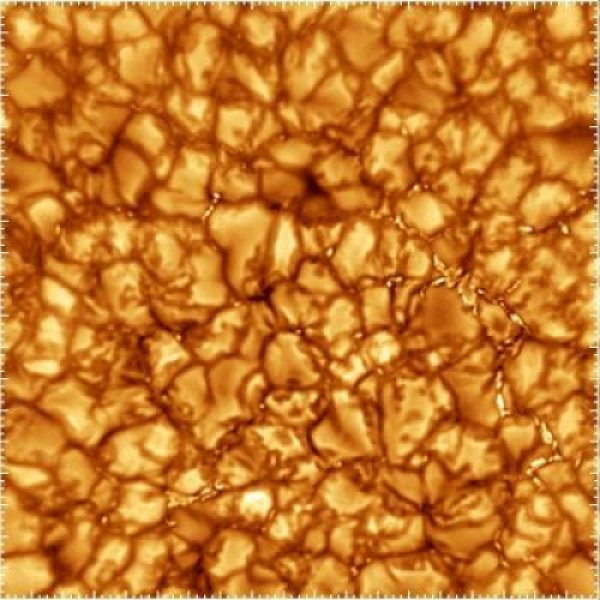
\includegraphics[height=3.5 cm]{media/granules.jpg}
\vspace*{-0.05in}
\flushright
\tiny{Max Planck Institute for Solar System Research \hspace*{3.6cm} BBSO/NJIT}
\end{frame}


\begin{frame}
\frametitle{Asymmetric magnetic slab}
\framesubtitle{Equilibrium conditions}
\begin{figure}
\centering
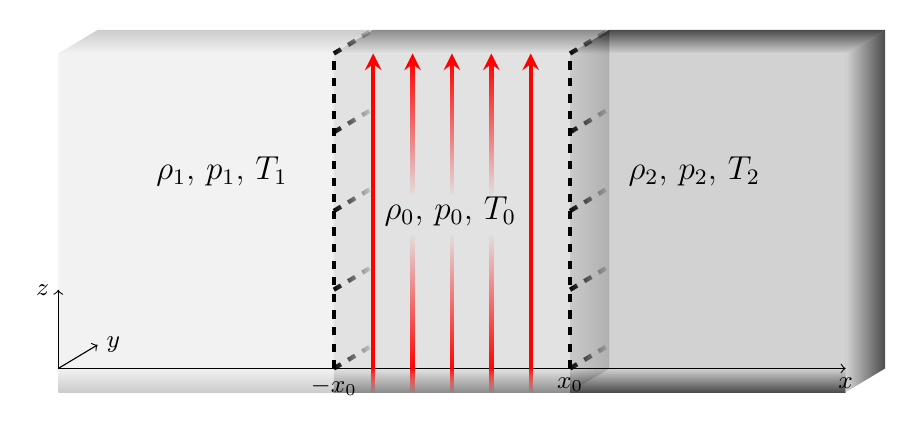
\begin{tikzpicture}
\path [fill=lightgray, opacity=0.45] (3.5,0) -- (3.5,4) -- (6.5,4) -- (6.5,0) -- (3.5,0);
\shade[left color=lightgray,right color=black, opacity=0.45] (6.5,0) -- (6.5,4) -- (7,4.3) -- (7,0.3) -- (6.5,0);
\shade[top color=lightgray,bottom color=black, opacity=0.45] (3.5,0) -- (6.5,0) -- (6.5,-0.3) -- (3.5,-0.3) -- (3.5,0);
\shade[top color=black,bottom color=lightgray, opacity=0.45] (3.5,4) -- (4,4.3) -- (7,4.3) -- (6.5,4) -- (3.5,4);
\shade[left color=lightgray,right color=black, opacity=0.45] (6.5,0) -- (6.5,-0.3) -- (7,0) -- (7,0.3) -- (6.5,0);

\path [fill=lightgray, opacity=0.7] (6.5,0) -- (6.5,4) -- (10,4) -- (10,0) -- (6.5,0);
\shade[top color=lightgray,bottom color=black, opacity=0.7] (6.5,0) -- (10,0) -- (10,-0.3) -- (6.5,-0.3) -- (6.5,0);
\shade[top color=black,bottom color=lightgray, opacity=0.7] (6.5,4) -- (7,4.3) -- (10.5,4.3) -- (10,4) -- (6.5,4);
\shade[left color=lightgray,right color=black, opacity=0.7] (10,-0.3) -- (10,4) -- (10.5,4.3) -- (10.5,0) -- (10,-0.3);

\path [fill=lightgray, opacity=0.2] (0,0) -- (0,4) -- (3.5,4) -- (3.5,0) -- (0,0);
\shade[top color=lightgray,bottom color=black, opacity=0.2] (0,0) -- (3.5,0) -- (3.5,-0.3) -- (0,-0.3) -- (0,0);
\shade[top color=black,bottom color=lightgray, opacity=0.2] (0,4) -- (0.5,4.3) -- (4,4.3) -- (3.5,4) -- (0,4);

\draw [<->] (0,1) -- (0,0) -- (10,0);
\draw [->] (0,0) -- (0.5,0.3);

\draw [ultra thick, dashed] (3.5,0) -- (3.5,4);
\draw [ultra thick, dashed, path fading=east] (3.5,0) -- (4,0.3);
\draw [ultra thick, dashed, path fading=east] (3.5,4) -- (4,4.3);
\draw [ultra thick, dashed, path fading=east] (3.5,2) -- (4,2.3);
\draw [ultra thick, dashed, path fading=east] (3.5,1) -- (4,1.3);
\draw [ultra thick, dashed, path fading=east] (3.5,3) -- (4,3.3);
\draw [ultra thick, red, -stealth] (4,0) -- (4,4);
\draw [ultra thick, red, path fading=south] (4,-0.3) -- (4,0);
\draw [ultra thick, red, path fading=north] (4.5,0) -- (4.5, 1.7);
\draw [ultra thick, red, path fading=south] (4.5,-0.3) -- (4.5,0);
\draw [ultra thick, red, path fading=south] (4.5,2.2) -- (4.5,3.9);
\draw [ultra thick, red, -stealth] (4.5,3.9) -- (4.5,4);
\draw [ultra thick, red, path fading=north] (5,0) -- (5, 1.7);
\draw [ultra thick, red, path fading=south] (5,-0.3) -- (5, 0);
\draw [ultra thick, red, path fading=south] (5,2.2) -- (5,3.9);
\draw [ultra thick, red, -stealth] (5,3.9) -- (5,4);
\draw [ultra thick, red, path fading=north] (5.5,0) -- (5.5, 1.7);
\draw [ultra thick, red, path fading=south] (5.5,-0.3) -- (5.5, 0);
\draw [ultra thick, red, path fading=south] (5.5,2.2) -- (5.5,3.9);
\draw [ultra thick, red, -stealth] (5.5,3.9) -- (5.5,4);
\draw [ultra thick, red, -stealth] (6,0) -- (6,4);
\draw [ultra thick, red, path fading=south] (6,-0.3) -- (6,0);
\draw [ultra thick, dashed] (6.5,0) --(6.5,4);
\draw [ultra thick, dashed, path fading=east] (6.5,0) -- (7,0.3);
\draw [ultra thick, dashed, path fading=east] (6.5,4) -- (7,4.3);
\draw [ultra thick, dashed, path fading=east] (6.5,2) -- (7,2.3);
\draw [ultra thick, dashed, path fading=east] (6.5,1) -- (7,1.3);
\draw [ultra thick, dashed, path fading=east] (6.5,3) -- (7,3.3);

\small
\node [below] at (3.5,0) {$-x_0$};
\node [below] at (6.5,0) {$x_0$};
\node [below] at (10,0) {$x$};
\node [left] at (0,1) {$z$};
\node [right] at (0.5,0.3) {$y$};

\large
\node [right] at (1.1,2.5) {$\rho_1$, $p_1$, $T_1$};
\node [right] at (4,2) {$\rho_0$, $p_0$, $T_0$};
\node [right] at (7.1,2.5) {$\rho_2$, $p_2$, $T_2$};
\end{tikzpicture}
\end{figure}

\begin{itemize}
  \item Uniform magnetic field in the slab.
  \item Field-free plasma outside.
  \item \textcolor{red}{Different} density and pressure on each side.
\end{itemize}
\end{frame}

\begin{frame}
\frametitle{Asymmetric magnetic slab}
\framesubtitle{Governing equations}
Ideal MHD equations: \hspace{3.8cm} Conservation of:
\begin{align*}
\rho\frac{\textrm{D}\boldsymbol{v}}{\textrm{D}{t}}&=-\nabla{p}-\frac{1}{\mu}\boldsymbol{B}\times(\nabla\times\boldsymbol{B}), & \text{momentum} \\
\frac{\partial\rho}{\partial{t}}+\nabla\cdot(\rho\boldsymbol{v})&=0, & \text{mass} \\
\frac{\textrm{D}}{\textrm{D}{t}}\left(\frac{p}{\rho^\gamma}\right)&=0, & \text{energy} \\
\frac{\partial{\boldsymbol{B}}}{\partial{t}}&=\nabla\times(\boldsymbol{v}\times\boldsymbol{B}), & \text{magnetic flux} 
\end{align*}

\small
\centering
\vspace{0.7cm}
\begin{tabular}{ll}
$\boldsymbol{v}=$ plasma velocity, & $\boldsymbol{B}=$ magnetic field strength,
\\
$\rho=$~density, & $p=$~pressure,
\\
$\mu=$ magnetic permeability, & $\gamma=$ adiabatic index.
\end{tabular}
\end{frame}


\begin{frame}
\frametitle{Asymmetric magnetic slab}
\framesubtitle{Fourier decomposition}
Look for \emph{plane wave} solutions of the form:
\begin{equation*}
v_x(\mathbf{x},t)=\hat{v}_x(x)e^{i(kz-\omega{t})}, \quad
v_y(\mathbf{x},t)=0, \quad
v_z(\mathbf{x},t)=\hat{v}_z(x)e^{i(kz-\omega{t})},
\end{equation*}
to arrive at the following ODEs:
\begin{figure}
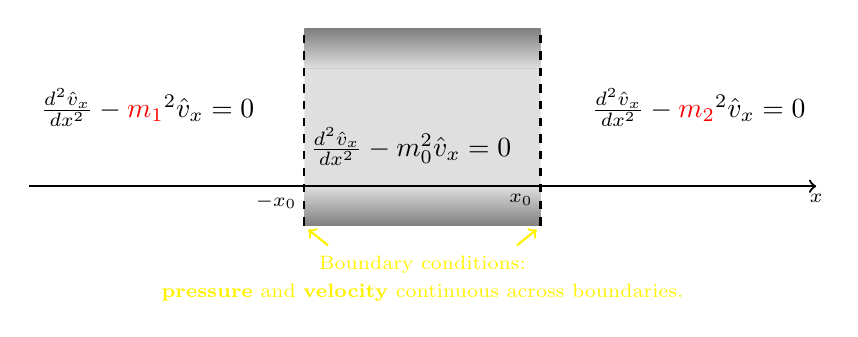
\begin{tikzpicture}
\path [fill=lightgray, opacity=0.5] (3.5,0) -- (3.5,1.5) -- (6.5,1.5) -- (6.5,0) -- (3.5,0);

\shade[bottom color=black,top color=lightgray, opacity=0.5] (3.5,-0.5) to (6.5,-0.5) to (6.5,0) to (3.5,0) to (3.5,-0.5);

\shade[top color=black,bottom color=lightgray, opacity=0.5] (3.5,2) to (6.5,2) to (6.5,1.5) to (3.5,1.5) to (3.5,2);

\draw [thick, dashed] (3.5,-0.5) -- (3.5,2);
\draw [thick, dashed] (6.5,-0.5) -- (6.5,2);

\draw [ thick, ->] (0,0) -- (10,0);
\scriptsize
\node [below] at (10,0) {$x$};

\scriptsize
\node [below left] at (3.5,0) {$-x_0$};
\node [below left] at (6.5,0) {$x_0$};

\normalsize
\node [right] at (3.45,0.5) {$\frac{d^2\hat{v}_x}{dx^2}-m_0^2\hat{v}_x=0$};
\node [right] at (0.03,1) {$\frac{d^2\hat{v}_x}{dx^2}-\textcolor{red}{m_1}^2\hat{v}_x=0$};
\node [right] at (7.03,1) {$\frac{d^2\hat{v}_x}{dx^2}-\textcolor{red}{m_2}^2\hat{v}_x=0$};

\scriptsize
\node at (5,-1) {\textcolor{yellow}{Boundary conditions:}};
\node at (5,-1.35) {\textcolor{yellow}{\textbf{pressure} and \textbf{velocity} continuous across boundaries.}};

\draw [thick, yellow, ->] (3.8,-0.75) -- (3.55, -0.55);
\draw [thick, yellow, ->] (6.2,-0.75) -- (6.45, -0.55);
\end{tikzpicture}
\end{figure}
\scriptsize
\begin{equation*}
{m_0}^2=\frac{(k^2{v_A}^2-\omega^2)(k^2c_0^2-\omega^2)}{(c_0^2+{v_A}^2)(k^2{c_T}^2-\omega^2)}, \qquad
\textcolor{red}{m_{1,2}}^2=k^2-\frac{\omega^2}{\textcolor{red}{c_{1,2}}^2},
\end{equation*}
\begin{equation*}
{c_T}^2=\frac{c_0^2{v_A}^2}{c_0^2+{v_A}^2}, \qquad {v_A}=\frac{{B_0}}{\sqrt{{\mu}\rho_0}},
\end{equation*}
\end{frame}


\begin{frame}
\frametitle{Asymmetric magnetic slab}
\framesubtitle{Eigenmodes}
\begin{block}{Dispersion relation:}
\vspace{-0.5cm}
\begin{align*}
&\frac{\omega^4{m_0}^2}{k^2{v_A}^2-\omega^2}+\frac{\rho_0}{\textcolor{red}{\rho_1}}\textcolor{red}{m_1}\frac{\rho_0}{\textcolor{red}{\rho_2}}\textcolor{red}{m_2}(k^2{v_A}^2-\omega^2) \\
&-\frac{1}{2}{m_0}\omega^2\left(\frac{\rho_0}{\textcolor{red}{\rho_1}}\textcolor{red}{m_1}+\frac{\rho_0}{\textcolor{red}{\rho_2}}\textcolor{red}{m_2}\right)\left(\tanh{{m_0}x_0}+\coth{{m_0}x_0}\right)=0,
\end{align*}
\end{block}
\scriptsize
See \textbf{Allcock} and Erd\'{e}lyi, 2017.
\begin{equation*}
{m_0}^2=\frac{(k^2{v_A}^2-\omega^2)(k^2c_0^2-\omega^2)}{(c_0^2+{v_A}^2)(k^2{c_T}^2-\omega^2)}, \qquad
\textcolor{red}{m_{1,2}}^2=k^2-\frac{\omega^2}{\textcolor{red}{c_{1,2}}^2},
\end{equation*}
\begin{equation*}
{c_T}^2=\frac{c_0^2{v_A}^2}{c_0^2+{v_A}^2}, \qquad {v_A}=\frac{{B_0}}{\sqrt{{\mu}\rho_0}},
\end{equation*}
\end{frame}
%
%
%
%
%
%
%
%
%
%
%
%
%
%%
%%
%%\begin{frame}
%%\frametitle{Asymmetric magnetic slab}
%%\frametitle{Eigenmodes - quasi-kink}
%%\begin{figure}
%%\hspace*{-1cm}
%%\includemedia[
%%  height=0.7\paperheight,
%%  transparent,
%%  addresource=media/R1_1.9_slow-kink-surf_mag_front_video_overlay2_looped.mp4,
%%  flashvars={
%%     source=media/R1_1.9_slow-kink-surf_mag_front_video_overlay2_looped.mp4
%%    &loop=true
%%  }
%%]{\centering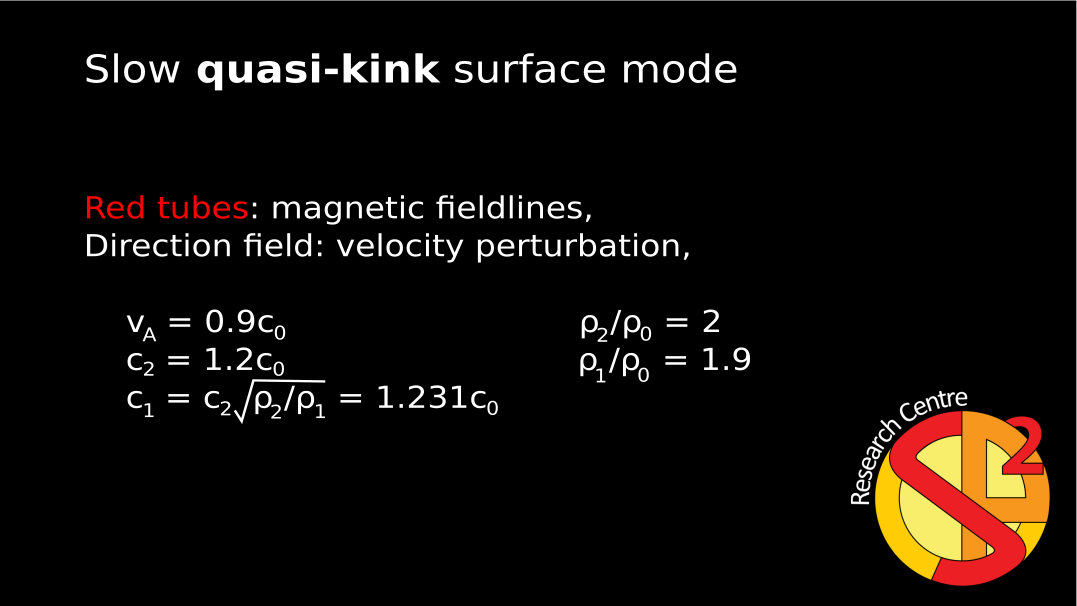
\includegraphics{media/animation-coverpage-slow-kink-surf.png}}{VPlayer.swf}
%%\end{figure}
%%\end{frame}
%%
%%
%%\begin{frame}
%%\frametitle{Asymmetric magnetic slab}
%%\frametitle{Eigenmodes - quasi-sausage}
%%\begin{figure}
%%\hspace*{-1cm}
%%\includemedia[
%%  height=0.7\paperheight,
%%  transparent,
%%  addresource=media/R1_1.9_slow-saus-surf_mag_front_video_overlay2_looped.mp4,
%%  flashvars={
%%     source=media/R1_1.9_slow-saus-surf_mag_front_video_overlay2_looped.mp4
%%    &loop=true
%%  }
%%]{\centering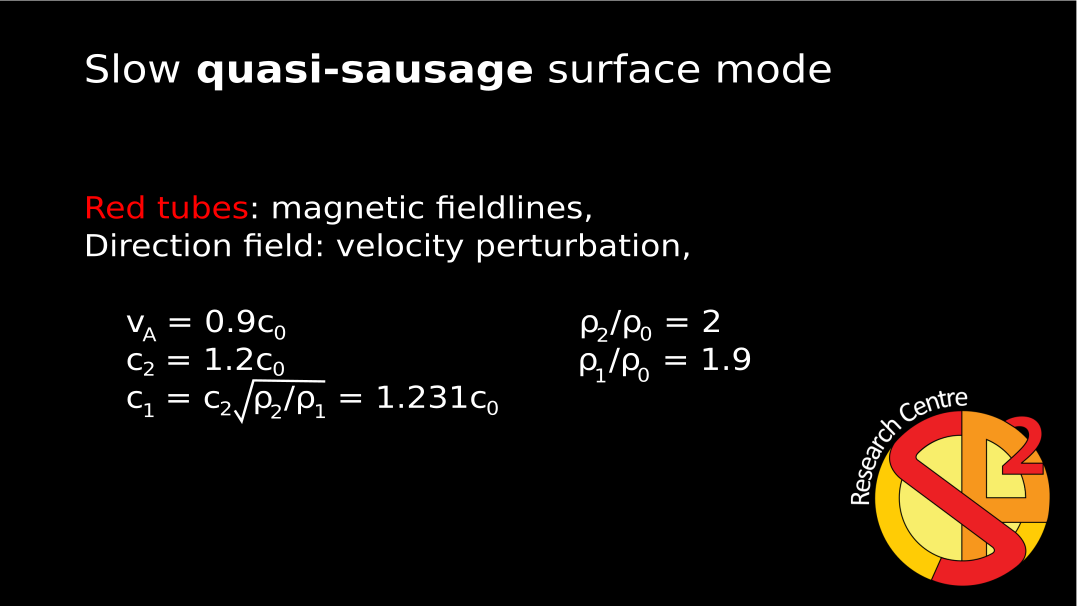
\includegraphics{media/animation-coverpage-slow-saus-surf.png}}{VPlayer.swf}
%%\end{figure}
%%\end{frame}
%%
%%
%%\begin{frame}
%%\frametitle{Asymmetric magnetic slab}
%%\frametitle{Eigenmodes - exotic modes}
%%%\begin{center}
%%\vspace*{-0.25in}
%%\begin{figure}
%%\makebox[\textwidth][c]{
%%\subfloat[]{
%%\includemedia[
%%  label=vidA,
%%  width=0.49\paperwidth,
%%  transparent,
%%  addresource=media/R1_1.8_fast-kink-body-1_front_video_overlay2_looped.mp4,
%%  flashvars={
%%     source=media/R1_1.8_fast-kink-body-1_front_video_overlay2_looped.mp4
%%    &loop=true
%%  }
%%]{\centering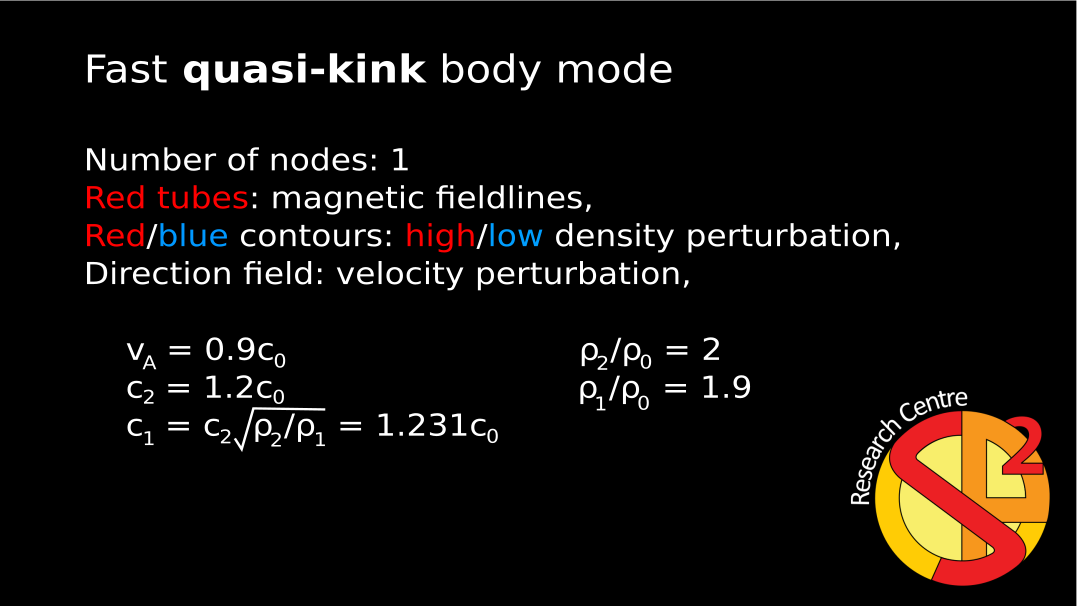
\includegraphics{media/animation-coverpage-fast-kink-body1.png}}{VPlayer.swf}
%%}
%%
%%\hspace*{-0.2in}
%%%\vspace*{-0.4in}
%%
%%\subfloat[]{
%%\includemedia[
%%  label=vidB,
%%  width=0.49\paperwidth,
%%  transparent,
%%  addresource=media/R1_1.8_fast-saus-body-1_front_video_overlay2_looped.mp4,
%%  flashvars={
%%     source=media/R1_1.8_fast-saus-body-1_front_video_overlay2_looped.mp4
%%    &loop=true
%%  }
%%]{\centering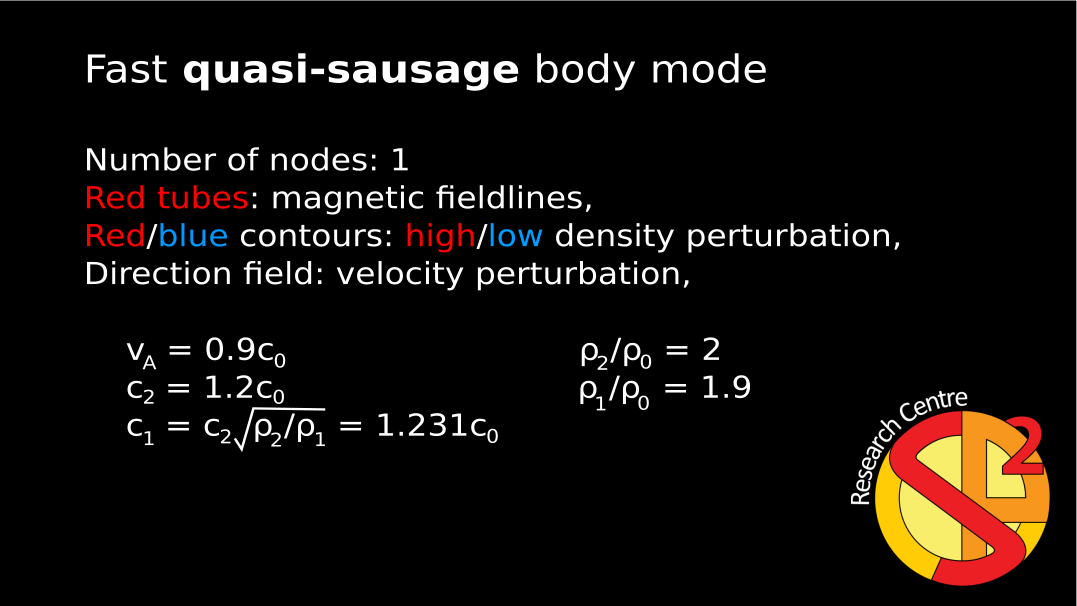
\includegraphics{media/animation-coverpage-fast-saus-body1.png}}{VPlayer.swf}
%%}}
%%
%%\vspace*{-0.1in}
%%
%%\makebox[\textwidth][c]{
%%\subfloat[]{
%%\includemedia[
%%  label=vidC,
%%  width=0.49\paperwidth,
%%  transparent,
%%  addresource=media/R1_1.8_fast-kink-body-2_front_video_overlay2_looped.mp4,
%%  flashvars={
%%     source=media/R1_1.8_fast-kink-body-2_front_video_overlay2_looped.mp4
%%    &loop=true
%%  }
%%]{\centering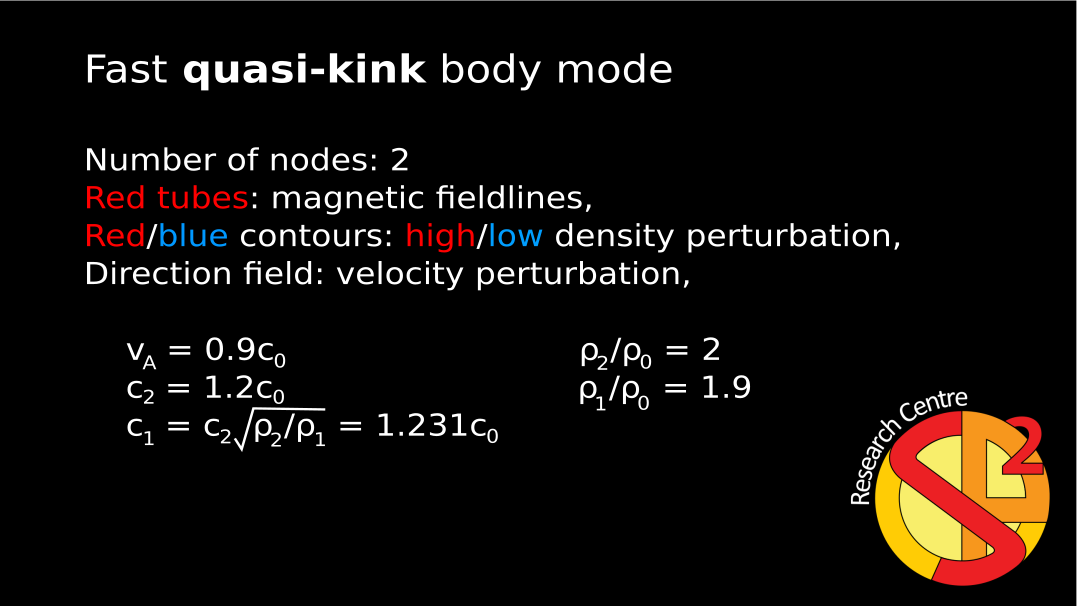
\includegraphics{media/animation-coverpage-fast-kink-body2.png}}{VPlayer.swf}
%%}
%%
%%\hspace*{-0.2in}
%%
%%\subfloat[]{
%%\includemedia[
%%  label=vidD,
%%  width=0.49\paperwidth,
%%  transparent,
%%  addresource=media/R1_1.8_fast-saus-body-2_front_video_overlay2_looped.mp4,
%%  flashvars={
%%     source=media/R1_1.8_fast-saus-body-2_front_video_overlay2_looped.mp4
%%    &loop=true
%%  }
%%]{\centering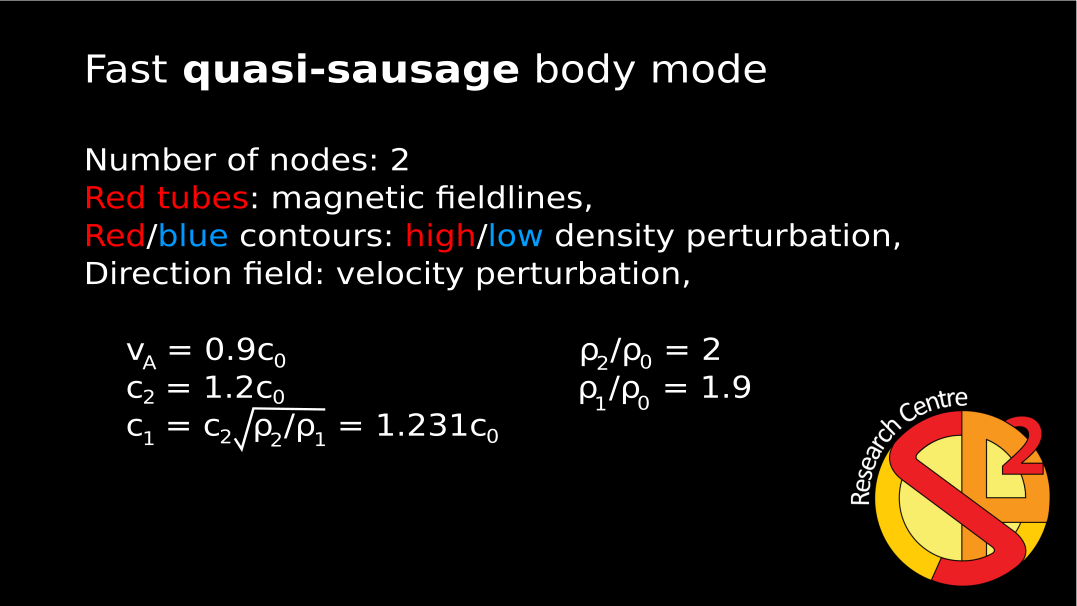
\includegraphics{media/animation-coverpage-fast-saus-body2.png}}{VPlayer.swf}
%%}}
%%\end{figure}
%%%\end{center}
%%
%%\vspace*{-0.4in}
%%
%%\mediabutton[
%%  mediacommand=vidA:playPause,
%%  mediacommand=vidB:playPause,
%%  mediacommand=vidC:playPause,
%%  mediacommand=vidD:playPause
%%]{\fbox{}}
%%\end{frame}
%%
%%
%%

\subsection{Mode identification}


\begin{frame}
\frametitle{Asymmetric magnetic slab}
\framesubtitle{Mode identification}
\centering
\large
Superposition of symmetric kink and sausage modes...
\begin{figure}
\centering
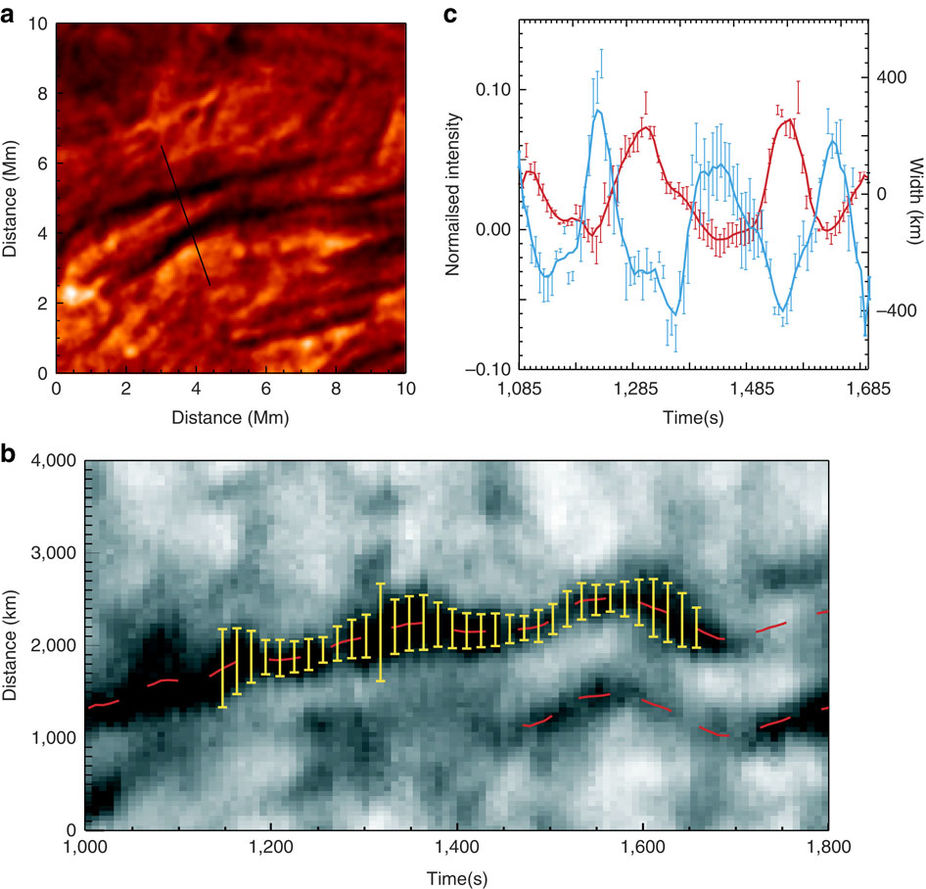
\includegraphics[height=5cm]{media/mor12.jpg}
\end{figure}
\tiny
\flushright{Morton \textit{et al.} 2012}\\
\normalsize
\centering
\pause
\large
or asymmetric kink mode?
\end{frame}


\subsection{Amplitude ratio}


\begin{frame}
\frametitle{Amplitude ratio}
\begin{figure}
\centering
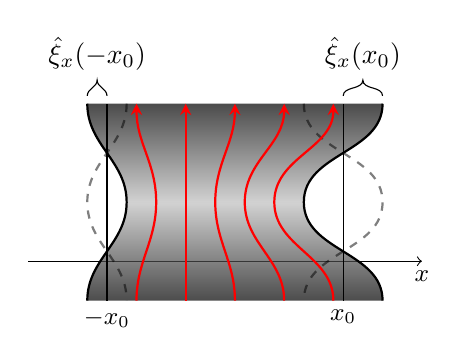
\begin{tikzpicture}
\draw [->] (1,0) -- (6,0);

\shade[bottom color=lightgray,top color=black, opacity=0.7] (1.75,2) to [out=-90,in=90] (2.25,0.75) to (4.5,0.75) to [out=90,in=-90] (5.5,2) to (1.75,2);

\shade[bottom color=black,top color=lightgray, opacity=0.7] (2.25,0.75) to (4.5,0.75) to [out=-90,in=90] (5.5,-0.5) to (1.75,-0.5) to [out=90,in=-90] (2.25,0.75);

\draw [thick] (1.75,2) to [out=-90,in=90] (2.25,0.75) to [out=-90,in=90] (1.75,-0.5);
\draw [thick, dashed, opacity=0.5] (4.5,2) to [out=-90,in=90] (5.5,0.75) to [out=-90,in=90] (4.5,-0.5);

\draw [thick, red, -stealth] (2.375,-0.5) to [out=90,in=-90] (2.625, 0.75) to [out=90,in=-90] (2.375,2);
\draw [thick, red, -stealth] (3,-0.5) to [out=90,in=-90] (3, 0.75) to [out=90,in=-90] (3,2);
\draw [thick, red, -stealth] (3.625,-0.5) to [out=90,in=-90] (3.375, 0.75) to [out=90,in=-90] (3.625,2);
\draw [thick, red, -stealth] (4.25,-0.5) to [out=90,in=-90] (3.75, 0.75) to [out=90,in=-90] (4.25,2);
\draw [thick, red, -stealth] (4.875,-0.5) to [out=90,in=-90] (4.125, 0.75) to [out=90,in=-90] (4.875,2);

\draw [thick, dashed, opacity=0.5] (2.25,2) to [out=-90,in=90] (1.75,0.75) to [out=-90,in=90] (2.25,-0.5);
\draw [thick] (5.5,2) to [out=-90,in=90] (4.5,0.75) to [out=-90,in=90] (5.5,-0.5);

% % % % % % % % % % % % % % % % % % % % % % % % % %

%\draw [->] (0,0) -- (0,2);

%\node at (1,1) {$\rho_1$};
%\node at (6,1) {$\rho_2$};
%\node [right] at (2.95,1.3) {$\rho_0$};

\draw [-] (1.75, 2.1) to [out=90, in=-90] (1.875, 2.3) to [out=-90, in=90] (2, 2.1);
\draw [-] (5, 2.1) to [out=90, in=-90] (5.25, 2.3) to [out=-90, in=90] (5.5, 2.1);

\node [above] at (1.875,2.3) {$\hat{\xi}_x(-x_0)$};
\node [above] at (5.25, 2.3) {$\hat{\xi}_x(x_0)$};

\small
\node [below] at (2,-0.5) {$-x_0$};
\node [below] at (5,-0.5) {$x_0$};

%\node [left] at (0,2) {$z$};
\node [below] at (6,0) {$x$};
\draw [-] (2,-0.5) -- (2,2);
\draw [-] (5,-0.5) -- (5,2);
\end{tikzpicture}
\end{figure}
\vspace{-0.3cm}
\begin{block}{Amplitude ratio}
\vspace{-0.3cm}
\begin{align*}
R_A :=& \frac{\hat{\xi}_x(x_0)}{\hat{\xi}_x(-x_0)} \qquad \qquad \qquad \qquad \qquad \left(\substack{\text{\textcolor{blue}{\tiny Top = quasi-kink}} \\ \text{\tiny \textcolor{red}{Bottom = quasi-sausage}}}\right)\\
=&\left(\substack{\textcolor{blue}{+} \\ \textcolor{red}{-}}\right) \frac{\rho_1m_2}{\rho_2m_1}\frac{(k^2{v_A}^2-\omega^2)m_1\frac{\rho_0}{\rho_1}-\omega^2{m_0}\left(\substack{\textcolor{blue}{\tanh} \\ \textcolor{red}{\coth}}\right){({m_0}x_0)}}{(k^2{v_A}^2-\omega^2)m_2\frac{\rho_0}{\rho_2}-\omega^2{m_0}\left(\substack{\textcolor{blue}{\tanh} \\ \textcolor{red}{\coth}}\right){({m_0}x_0)}}
\end{align*}
\end{block}
\end{frame}

\begin{frame}
\frametitle{Amplitude ratio}
\framesubtitle{Parameter inversion}
\vspace*{-0.2in}
\begin{block}{Parameter inversion}
\begin{itemize}
\item \textbf{Observe}: $\omega$, $k$, $x_0$, $T_i$, and $R_\mathrm{A}$.
\item \textbf{Solve} to find: $\textcolor{red}{v_A}$ and hence $\textcolor{red}{B_0}$.
\end{itemize}
\end{block}

\begin{overlayarea}{\textwidth}{0.5\textheight}
\only<2>{
\huge
\centering
Analytical inversion
}

\only<3>{
\vspace*{0.5in}
\hspace*{-0.9cm}
\tiny
\begin{tabular}{llccc}
\toprule
Mode & \multicolumn{3}{c}{Approximation of $k^2\textcolor{red}{v_{\textrm{A}}}^2 / \omega^2$ using amplitude ratio, $R_{\textrm{A}}$} \\
\cmidrule(lr){2-4}
& \multicolumn{1}{c}{Thin slab} & \multicolumn{1}{c}{Incompressible} & \multicolumn{1}{c}{Low-beta} \\
\midrule
Sausage & $ 1 + \frac{1}{x_0}\left(\frac{R_{\textrm{A}}\frac{\rho_2}{\rho_0m_2} + \frac{\rho_1}{\rho_0m_1}}{R_{\textrm{A}} + 1}\right) $ & $ 1 + \left( \frac{R_{\textrm{A}} \frac{\rho_2}{\rho_0} + \frac{\rho_1}{\rho_0}}{R_{\textrm{A}} + 1} \right) \coth{kx_0} $ & $ 1 + k \left( \frac{ R_{\textrm{A}}\frac{\rho_2}{\rho_0m_2} + \frac{\rho_1}{\rho_0m_1}}{R_{\textrm{A}} + 1} \right) \coth{kx_0} $ \\
Kink	   & $ 1 + k^2x_0\left(\frac{R_{\textrm{A}}\frac{\rho_2}{\rho_0m_2} - \frac{\rho_1}{\rho_0m_1}}{R_{\textrm{A}} - 1}\right) $ & $ 1 + \left( \frac{R_{\textrm{A}} \frac{\rho_2}{\rho_0} - \frac{\rho_1}{\rho_0}}{R_{\textrm{A}} - 1} \right) \tanh{kx_0} $ & $ 1 + k \left( \frac{ R_{\textrm{A}}\frac{\rho_2}{\rho_0m_2} - \frac{\rho_1}{\rho_0m_1}}{R_{\textrm{A}} - 1} \right) \tanh{kx_0} $ \\
\bottomrule
\end{tabular}
}

\only<4>{
\huge
\centering
Numerical inversion
}

\only<5>{
%\vspace*{-1.4in}
\centering
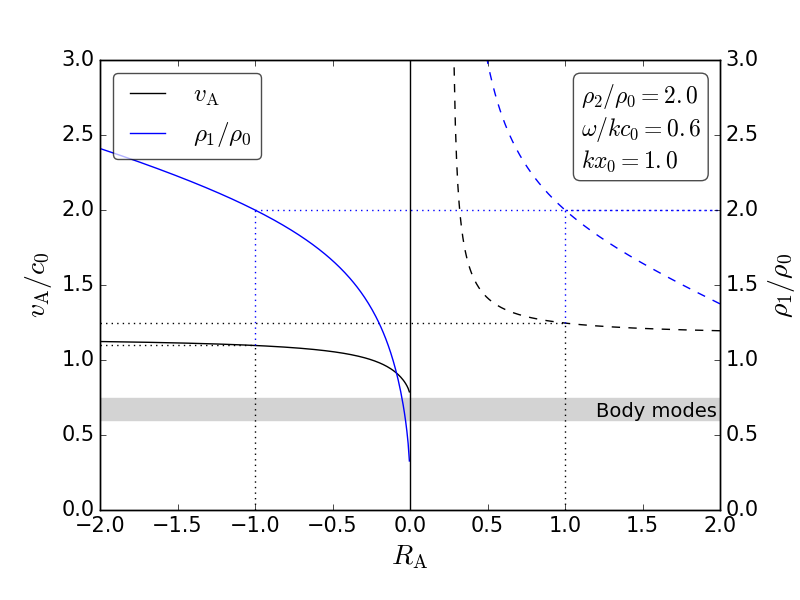
\includegraphics[height=6cm]{media/RA_vA_approx_2var.png}
}
\end{overlayarea}
\end{frame}


\subsection{Minimum perturbation shift}


\begin{frame}
\frametitle{Minimum perturbation shift}
\begin{figure}
\centering
\makebox[\textwidth][c]{
\subfloat[]{\scalebox{0.9}{
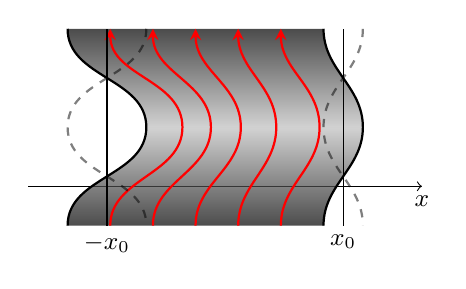
\begin{tikzpicture}
\draw [->] (1,0) -- (6,0);

\shade[bottom color=lightgray,top color=black, opacity=0.7] (1.5,2) to [out=-90,in=90] (2.5,0.75) to (5.25,0.75) to [out=90,in=-90] (4.75,2) to (1.5,2);

\shade[bottom color=black,top color=lightgray, opacity=0.7] (2.5,0.75) to (5.25,0.75) to [out=-90,in=90] (4.75,-0.5) to (1.5,-0.5) to [out=90,in=-90] (2.5,0.75);

\draw [thick] (1.5,2) to [out=-90,in=90] (2.5,0.75) to [out=-90,in=90] (1.5,-0.5);
\draw [thick] (4.75,2) to [out=-90,in=90] (5.25,0.75) to [out=-90,in=90] (4.75,-0.5);

%\draw [thick, red, -stealth] (2.0417,-0.5) to [out=90,in=-90] (2.9583, 0.75) to [out=90,in=-90] (2.0417,2);
%\draw [thick, red, -stealth] (2.5833,-0.5) to [out=90,in=-90] (3.4167, 0.75) to [out=90,in=-90] (2.5833,2);
%\draw [thick, red, -stealth] (3.125,-0.5) to [out=90,in=-90] (3.875, 0.75) to [out=90,in=-90] (3.125,2);
%\draw [thick, red, -stealth] (3.6667,-0.5) to [out=90,in=-90] (4.3333, 0.75) to [out=90,in=-90] (3.6667,2);
%\draw [thick, red, -stealth] (4.2083,-0.5) to [out=90,in=-90] (4.7917, 0.75) to [out=90,in=-90] (4.2083,2);

\draw [thick, red, -stealth] (2.0417,-0.5) to [out=90,in=-90] (2.9583, 0.75) to [out=90,in=-90] (2.0417,2);
\draw [thick, red, -stealth] (2.5833,-0.5) to [out=90,in=-90] (3.32, 0.75) to [out=90,in=-90] (2.5833,2);
\draw [thick, red, -stealth] (3.125,-0.5) to [out=90,in=-90] (3.7, 0.75) to [out=90,in=-90] (3.125,2);
\draw [thick, red, -stealth] (3.6667,-0.5) to [out=90,in=-90] (4.15, 0.75) to [out=90,in=-90] (3.6667,2);
\draw [thick, red, -stealth] (4.2083,-0.5) to [out=90,in=-90] (4.7, 0.75) to [out=90,in=-90] (4.2083,2);

\draw [thick, dashed, opacity=0.5] (2.5,2) to [out=-90,in=90] (1.5,0.75) to [out=-90,in=90] (2.5,-0.5);
\draw [thick, dashed, opacity=0.5] (5.25,2) to [out=-90,in=90] (4.75,0.75) to [out=-90,in=90] (5.25,-0.5);

% % % % % % % % % % % % % % % % % % % % % % % % % %

%\draw [->] (0,0) -- (0,2);

%\node at (1,1) {$\rho_1$};
%\node at (6,1) {$\rho_2$};
%\node at (3.6,0.8) {$\rho_0$};

\small
\node [below] at (2,-0.5) {$-x_0$};
\node [below] at (5,-0.5) {$x_0$};

%\node [left] at (0,2) {$z$};
\node [below] at (6,0) {$x$};
\draw [-] (2,-0.5) -- (2,2);
\draw [-] (5,-0.5) -- (5,2);
\end{tikzpicture}
}}


\subfloat[]{\scalebox{0.9}{
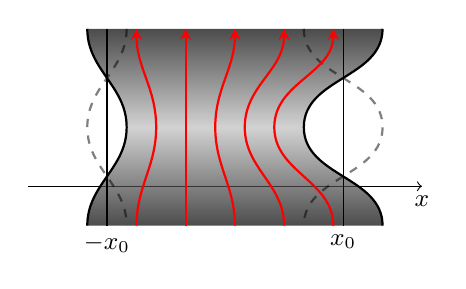
\begin{tikzpicture}
\draw [->] (1,0) -- (6,0);

\shade[bottom color=lightgray,top color=black, opacity=0.7] (1.75,2) to [out=-90,in=90] (2.25,0.75) to (4.5,0.75) to [out=90,in=-90] (5.5,2) to (1.75,2);

\shade[bottom color=black,top color=lightgray, opacity=0.7] (2.25,0.75) to (4.5,0.75) to [out=-90,in=90] (5.5,-0.5) to (1.75,-0.5) to [out=90,in=-90] (2.25,0.75);

\draw [thick] (1.75,2) to [out=-90,in=90] (2.25,0.75) to [out=-90,in=90] (1.75,-0.5);
\draw [thick, dashed, opacity=0.5] (4.5,2) to [out=-90,in=90] (5.5,0.75) to [out=-90,in=90] (4.5,-0.5);

\draw [thick, red, -stealth] (2.375,-0.5) to [out=90,in=-90] (2.625, 0.75) to [out=90,in=-90] (2.375,2);
\draw [thick, red, -stealth] (3,-0.5) to [out=90,in=-90] (3, 0.75) to [out=90,in=-90] (3,2);
\draw [thick, red, -stealth] (3.625,-0.5) to [out=90,in=-90] (3.375, 0.75) to [out=90,in=-90] (3.625,2);
\draw [thick, red, -stealth] (4.25,-0.5) to [out=90,in=-90] (3.75, 0.75) to [out=90,in=-90] (4.25,2);
\draw [thick, red, -stealth] (4.875,-0.5) to [out=90,in=-90] (4.125, 0.75) to [out=90,in=-90] (4.875,2);

\draw [thick, dashed, opacity=0.5] (2.25,2) to [out=-90,in=90] (1.75,0.75) to [out=-90,in=90] (2.25,-0.5);
\draw [thick] (5.5,2) to [out=-90,in=90] (4.5,0.75) to [out=-90,in=90] (5.5,-0.5);

% % % % % % % % % % % % % % % % % % % % % % % % % %

%\draw [->] (0,0) -- (0,2);

%\node at (1,1) {$\rho_1$};
%\node at (6,1) {$\rho_2$};
%\node [right] at (2.95,1.3) {$\rho_0$};

%\draw [-] (1.75, 2.1) to [out=90, in=-90] (1.875, 2.3) to [out=-90, in=90] (2, 2.1);

%\node [above] at (1.875,2.3) {$\hat{v}_x(-x_0)$};
%\node [above] at (5.25, 2.3) {$\hat{v}_x(x_0)$};

\small
\node [below] at (2,-0.5) {$-x_0$};
\node [below] at (5,-0.5) {$x_0$};

%\node [left] at (0,2) {$z$};
\node [below] at (6,0) {$x$};
\draw [-] (2,-0.5) -- (2,2);
\draw [-] (5,-0.5) -- (5,2);
\end{tikzpicture}
}}}

\vspace*{-0.5cm}

\makebox[\textwidth][c]{
\subfloat[]{\scalebox{0.9}{
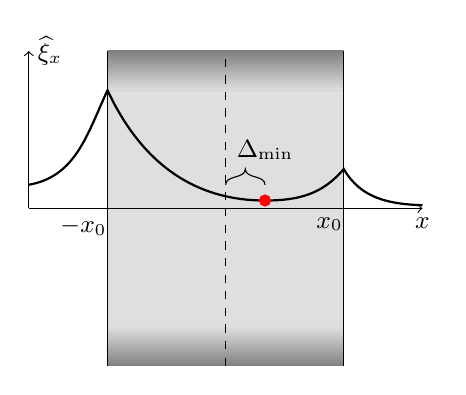
\begin{tikzpicture}
\path [fill=lightgray, opacity=0.5] (2,-1.5) -- (2,1.5) -- (5,1.5) -- (5,-1.5) -- (2,-1.5);

\shade[bottom color=black,top color=lightgray, opacity=0.5] (2,-2) to (5,-2) to (5,-1.5) to (2,-1.5) to (2,-2);

\shade[top color=black,bottom color=lightgray, opacity=0.5] (2,2) to (5,2) to (5,1.5) to (2,1.5) to (2,2);

\draw [-] (2,-2) -- (2,2);
\draw [-] (5,-2) -- (5,2);

%\draw [ultra thick, red, -stealth,opacity=0.7] (2.5,-1.5) -- (2.5,2);
%\draw [ultra thick, red, path fading=south, opacity=0.5] (2.5,-2) -- (2.5,-1.5);
%\draw [ultra thick, red, -stealth,opacity=0.7] (3,-1.5) -- (3,2);
%\draw [ultra thick, red, path fading=south,opacity=0.5] (3,-2) -- (3,-1.5);
%\draw [ultra thick, red, -stealth,opacity=0.7] (3.5,-1.5) -- (3.5,2);
%\draw [ultra thick, red, path fading=south,opacity=0.5] (3.5,-2) -- (3.5,-1.5);
%\draw [ultra thick, red, -stealth,opacity=0.7] (4,-1.5) -- (4,2);
%\draw [ultra thick, red, path fading=south,opacity=0.5] (4,-2) -- (4,-1.5);
%\draw [ultra thick, red, -stealth,opacity=0.7] (4.5,-1.5) -- (4.5,2);
%\draw [ultra thick, red, path fading=south,opacity=0.5] (4.5,-2) -- (4.5,-1.5);

%\draw [thick] (0,0.2) to [out=10, in=245] (2, 1.5) to [out=295, in=180] (4,0.1) to [out=0, in=230] (5,0.5) to [out=300, in=178] (6.2,0.04) to [out=358, in=180] (7,0.02);

\draw [thick] (1,0.3) to [out=10, in=245] (2, 1.5) to [out=295, in=180] (4,0.1) to [out=0, in=230] (5,0.5) to [out=300, in=178] (6,0.04);

\draw [->] (1,0) -- (1,2);
\draw [->] (1,0) -- (6,0);
%
%\node at (1,1) {$\rho_1$};
%\node at (6,1) {$\rho_2$};
%\node [right] at (2.88,1.3) {$\rho_0$};

\small
\node [below left] at (2.1,0) {$-x_0$};
\node [below left] at (5.1,0) {$x_0$};

\node [right] at (1,2) {$\widehat{\xi}_x$};
\node [below] at (6,0) {$x$};

\draw [dashed] (3.5,-2) -- (3.5,2);
\draw [fill, red] (4,0.1) circle [radius=0.07];
\draw [-] (3.5, 0.3) to [out=90, in=-90] (3.75, 0.5) to [out=-90, in=90] (4, 0.3);
\node [above] at (4., 0.5) {$\Delta_\mathrm{min}$};
\end{tikzpicture}
}}




\subfloat[]{\scalebox{0.9}{
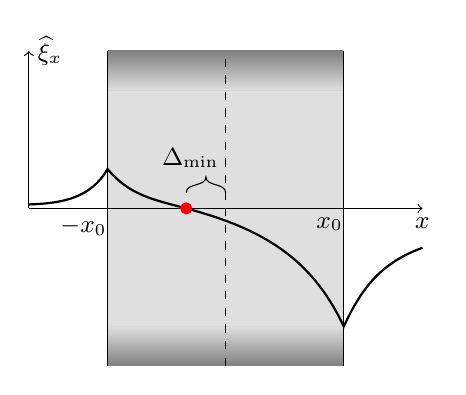
\begin{tikzpicture}
\path [fill=lightgray, opacity=0.5] (2,-1.5) -- (2,1.5) -- (5,1.5) -- (5,-1.5) -- (2,-1.5);

\shade[bottom color=black,top color=lightgray, opacity=0.5] (2,-2) to (5,-2) to (5,-1.5) to (2,-1.5) to (2,-2);

\shade[top color=black,bottom color=lightgray, opacity=0.5] (2,2) to (5,2) to (5,1.5) to (2,1.5) to (2,2);

\draw [-] (2,-2) -- (2,2);
\draw [-] (5,-2) -- (5,2);

%\draw [ultra thick, red, -stealth,opacity=0.7] (2.5,-1.5) -- (2.5,2);
%\draw [ultra thick, red, path fading=south, opacity=0.5] (2.5,-2) -- (2.5,-1.5);
%\draw [ultra thick, red, -stealth,opacity=0.7] (3,-1.5) -- (3,2);
%\draw [ultra thick, red, path fading=south,opacity=0.5] (3,-2) -- (3,-1.5);
%\draw [ultra thick, red, -stealth,opacity=0.7] (3.5,-1.5) -- (3.5,2);
%\draw [ultra thick, red, path fading=south,opacity=0.5] (3.5,-2) -- (3.5,-1.5);
%\draw [ultra thick, red, -stealth,opacity=0.7] (4,-1.5) -- (4,2);
%\draw [ultra thick, red, path fading=south,opacity=0.5] (4,-2) -- (4,-1.5);
%\draw [ultra thick, red, -stealth,opacity=0.7] (4.5,-1.5) -- (4.5,2);
%\draw [ultra thick, red, path fading=south,opacity=0.5] (4.5,-2) -- (4.5,-1.5);

%\draw [thick] (0,0.025) to [out=0, in=-178] (1.2, 0.05) to [out=2, in=-120] (2,0.5) to [out=-50, in=165] (3,0) to [out=-15, in=115] (5,-1.5) to [out=65, in=-170] (7,-0.2);

\draw [thick] (1, 0.05) to [out=2, in=-120] (2,0.5) to [out=-50, in=165] (3,0) to [out=-15, in=115] (5,-1.5) to [out=65, in=-160] (6,-0.5);

\draw [->] (1,0) -- (1,2);
\draw [->] (1,0) -- (6,0);

%\node at (1,1) {$\rho_1$};
%\node at (6,1) {$\rho_2$};
%\node [right] at (2.88,1.3) {$\rho_0$};

\small
\node [below left] at (2.1,0) {$-x_0$};
\node [below left] at (5.1,0) {$x_0$};

\node [right] at (1,2) {$\widehat{\xi}_x$};
\node [below] at (6,0) {$x$};

\draw [dashed] (3.5,-2) -- (3.5,2);
\draw [fill, red] (3,0) circle [radius=0.07];
\draw [-] (3, 0.2) to [out=90, in=-90] (3.25, 0.4) to [out=-90, in=90] (3.5, 0.2);
\node [above] at (3.05, 0.4) {$\Delta_\mathrm{min}$};
\end{tikzpicture}
}}}
\end{figure}
\end{frame}


\begin{frame}
\frametitle{Minimum perturbation shift}
\begin{figure}
\centering
\makebox[\textwidth][c]{
\subfloat[]{\scalebox{0.9}{
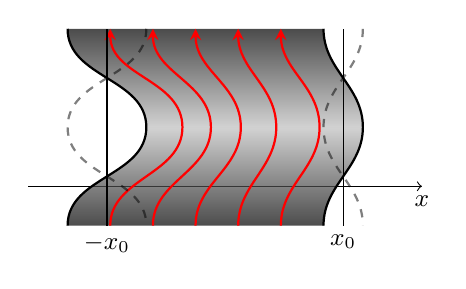
\begin{tikzpicture}
\draw [->] (1,0) -- (6,0);

\shade[bottom color=lightgray,top color=black, opacity=0.7] (1.5,2) to [out=-90,in=90] (2.5,0.75) to (5.25,0.75) to [out=90,in=-90] (4.75,2) to (1.5,2);

\shade[bottom color=black,top color=lightgray, opacity=0.7] (2.5,0.75) to (5.25,0.75) to [out=-90,in=90] (4.75,-0.5) to (1.5,-0.5) to [out=90,in=-90] (2.5,0.75);

\draw [thick] (1.5,2) to [out=-90,in=90] (2.5,0.75) to [out=-90,in=90] (1.5,-0.5);
\draw [thick] (4.75,2) to [out=-90,in=90] (5.25,0.75) to [out=-90,in=90] (4.75,-0.5);

%\draw [thick, red, -stealth] (2.0417,-0.5) to [out=90,in=-90] (2.9583, 0.75) to [out=90,in=-90] (2.0417,2);
%\draw [thick, red, -stealth] (2.5833,-0.5) to [out=90,in=-90] (3.4167, 0.75) to [out=90,in=-90] (2.5833,2);
%\draw [thick, red, -stealth] (3.125,-0.5) to [out=90,in=-90] (3.875, 0.75) to [out=90,in=-90] (3.125,2);
%\draw [thick, red, -stealth] (3.6667,-0.5) to [out=90,in=-90] (4.3333, 0.75) to [out=90,in=-90] (3.6667,2);
%\draw [thick, red, -stealth] (4.2083,-0.5) to [out=90,in=-90] (4.7917, 0.75) to [out=90,in=-90] (4.2083,2);

\draw [thick, red, -stealth] (2.0417,-0.5) to [out=90,in=-90] (2.9583, 0.75) to [out=90,in=-90] (2.0417,2);
\draw [thick, red, -stealth] (2.5833,-0.5) to [out=90,in=-90] (3.32, 0.75) to [out=90,in=-90] (2.5833,2);
\draw [thick, red, -stealth] (3.125,-0.5) to [out=90,in=-90] (3.7, 0.75) to [out=90,in=-90] (3.125,2);
\draw [thick, red, -stealth] (3.6667,-0.5) to [out=90,in=-90] (4.15, 0.75) to [out=90,in=-90] (3.6667,2);
\draw [thick, red, -stealth] (4.2083,-0.5) to [out=90,in=-90] (4.7, 0.75) to [out=90,in=-90] (4.2083,2);

\draw [thick, dashed, opacity=0.5] (2.5,2) to [out=-90,in=90] (1.5,0.75) to [out=-90,in=90] (2.5,-0.5);
\draw [thick, dashed, opacity=0.5] (5.25,2) to [out=-90,in=90] (4.75,0.75) to [out=-90,in=90] (5.25,-0.5);

% % % % % % % % % % % % % % % % % % % % % % % % % %

%\draw [->] (0,0) -- (0,2);

%\node at (1,1) {$\rho_1$};
%\node at (6,1) {$\rho_2$};
%\node at (3.6,0.8) {$\rho_0$};

\small
\node [below] at (2,-0.5) {$-x_0$};
\node [below] at (5,-0.5) {$x_0$};

%\node [left] at (0,2) {$z$};
\node [below] at (6,0) {$x$};
\draw [-] (2,-0.5) -- (2,2);
\draw [-] (5,-0.5) -- (5,2);
\end{tikzpicture}
}}


\subfloat[]{\scalebox{0.9}{
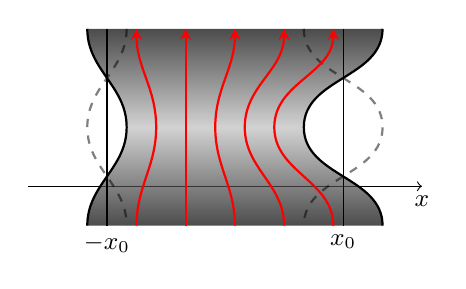
\begin{tikzpicture}
\draw [->] (1,0) -- (6,0);

\shade[bottom color=lightgray,top color=black, opacity=0.7] (1.75,2) to [out=-90,in=90] (2.25,0.75) to (4.5,0.75) to [out=90,in=-90] (5.5,2) to (1.75,2);

\shade[bottom color=black,top color=lightgray, opacity=0.7] (2.25,0.75) to (4.5,0.75) to [out=-90,in=90] (5.5,-0.5) to (1.75,-0.5) to [out=90,in=-90] (2.25,0.75);

\draw [thick] (1.75,2) to [out=-90,in=90] (2.25,0.75) to [out=-90,in=90] (1.75,-0.5);
\draw [thick, dashed, opacity=0.5] (4.5,2) to [out=-90,in=90] (5.5,0.75) to [out=-90,in=90] (4.5,-0.5);

\draw [thick, red, -stealth] (2.375,-0.5) to [out=90,in=-90] (2.625, 0.75) to [out=90,in=-90] (2.375,2);
\draw [thick, red, -stealth] (3,-0.5) to [out=90,in=-90] (3, 0.75) to [out=90,in=-90] (3,2);
\draw [thick, red, -stealth] (3.625,-0.5) to [out=90,in=-90] (3.375, 0.75) to [out=90,in=-90] (3.625,2);
\draw [thick, red, -stealth] (4.25,-0.5) to [out=90,in=-90] (3.75, 0.75) to [out=90,in=-90] (4.25,2);
\draw [thick, red, -stealth] (4.875,-0.5) to [out=90,in=-90] (4.125, 0.75) to [out=90,in=-90] (4.875,2);

\draw [thick, dashed, opacity=0.5] (2.25,2) to [out=-90,in=90] (1.75,0.75) to [out=-90,in=90] (2.25,-0.5);
\draw [thick] (5.5,2) to [out=-90,in=90] (4.5,0.75) to [out=-90,in=90] (5.5,-0.5);

% % % % % % % % % % % % % % % % % % % % % % % % % %

%\draw [->] (0,0) -- (0,2);

%\node at (1,1) {$\rho_1$};
%\node at (6,1) {$\rho_2$};
%\node [right] at (2.95,1.3) {$\rho_0$};

%\draw [-] (1.75, 2.1) to [out=90, in=-90] (1.875, 2.3) to [out=-90, in=90] (2, 2.1);

%\node [above] at (1.875,2.3) {$\hat{v}_x(-x_0)$};
%\node [above] at (5.25, 2.3) {$\hat{v}_x(x_0)$};

\small
\node [below] at (2,-0.5) {$-x_0$};
\node [below] at (5,-0.5) {$x_0$};

%\node [left] at (0,2) {$z$};
\node [below] at (6,0) {$x$};
\draw [-] (2,-0.5) -- (2,2);
\draw [-] (5,-0.5) -- (5,2);
\end{tikzpicture}
}}}
\end{figure}

\vspace{0.3cm}
\begin{block}{\textbf{Quasi-kink: \hspace{3.5cm} Quasi-sausage:}}
\vspace{-0.3cm}
\begin{equation*}
\Delta_\mathrm{min} = \frac{1}{m_0}\tanh^{-1}(D)
\hspace{2cm}
\Delta_\mathrm{min} = \frac{1}{m_0}\tanh^{-1}\left( \frac{1}{D} \right)
\end{equation*}
\end{block}

\begin{equation*}
\text{where} \quad
D = \frac{(k^2{v_A}^2-\omega^2)m_2\frac{\rho_0}{\rho_2}\tanh({m_0}x_0) - \omega^2{m_0}}{(k^2{v_A}^2-\omega^2)m_2\frac{\rho_0}{\rho_2} - \omega^2{m_0}\tanh({m_0}x_0)}
\end{equation*}
\end{frame}



\begin{frame}
\frametitle{Minimum perturbation shift}
\framesubtitle{Parameter inversion}
\vspace*{-0.2in}
\begin{block}{Parameter inversion}
\begin{itemize}
\item \textbf{Observe}: $\omega$, $k$, $x_0$, $T_i$, and $\Delta_\mathrm{min}$.
\item \textbf{Solve} to find: $\textcolor{red}{v_A}$ and hence $\textcolor{red}{B_0}$.
\end{itemize}
\end{block}

\begin{overlayarea}{\textwidth}{0.5\textheight}
\only<2>{
\huge
\centering
Analytical inversion
}

\only<3>{
\vspace*{0.5in}
\hspace*{-1.3cm}
\tiny
\begin{tabular}{llccc}
  \toprule
Mode & \multicolumn{3}{c}{Approximation of $k^2v_{\textrm{A}}^2 / \omega^2$ using minimum perturbation shift, $\Delta_{\textrm{min}}$} \\
\cmidrule(lr){2-4}
& Thin slab & Incompressible & Low-beta \\
  \midrule
Quasi-sausage & $ \frac{\rho_1}{\rho_0m_1}(x_0 + \Delta_{\textrm{min}}) + \frac{1}{1 + (\omega / kc_0)^2} + k^2x_0\Delta_{\textrm{min}} $ & $ 1 + \frac{\rho_1}{\rho_0}\tanh{k(x_0 + \Delta_{\textrm{min}})} $ & $ 1 + \frac{k\rho_1}{m_1\rho_0}\tanh{k(x_0 + \Delta_{\textrm{min}})} $ \\
Quasi-kink	   & $\frac{-b \pm \sqrt{b^2 - 4ac}}{2a}$, defined in text & $ 1 + \frac{\rho_1}{\rho_0}\coth{k(x_0 + \Delta_{\textrm{min}})} $ & $ 1 + \frac{k\rho_1}{m_1\rho_0}\coth{k(x_0 + \Delta_{\textrm{min}})} $ \\
  \bottomrule
\end{tabular}
}

\only<4>{
\huge
\centering
Numerical inversion
}

\only<5>{
%\vspace*{-1.4in}
\centering
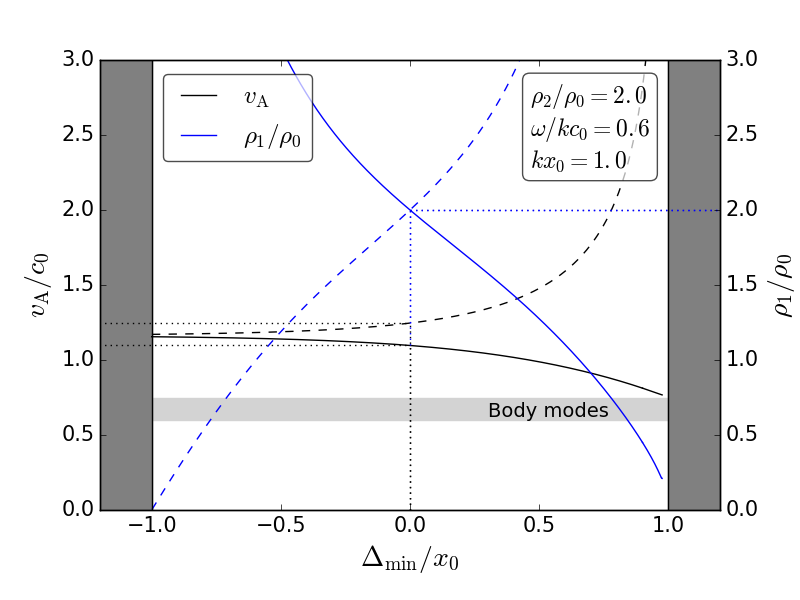
\includegraphics[height=6cm]{media/DM_vA_approx_2var.png}
}
\end{overlayarea}
\end{frame}


\section{Looking ahead}

\begin{frame}
\frametitle{Further work}
\framesubtitle{External magnetic field}
Add \textcolor{red}{\textbf{magnetic field}} outside the slab - coronal structures. See \textbf{Zs\'{a}mberger}, \textbf{Allcock} and \textbf{Erd\'{e}lyi}, submitted.

\begin{figure}
\centering
\scalebox{0.6}{
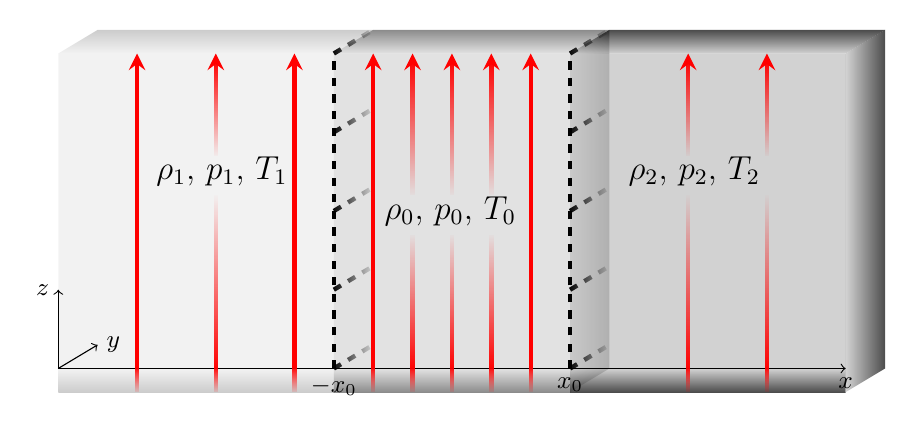
\begin{tikzpicture}
\path [fill=lightgray, opacity=0.45] (3.5,0) -- (3.5,4) -- (6.5,4) -- (6.5,0) -- (3.5,0);
\shade[left color=lightgray,right color=black, opacity=0.45] (6.5,0) -- (6.5,4) -- (7,4.3) -- (7,0.3) -- (6.5,0);
\shade[top color=lightgray,bottom color=black, opacity=0.45] (3.5,0) -- (6.5,0) -- (6.5,-0.3) -- (3.5,-0.3) -- (3.5,0);
\shade[top color=black,bottom color=lightgray, opacity=0.45] (3.5,4) -- (4,4.3) -- (7,4.3) -- (6.5,4) -- (3.5,4);
\shade[left color=lightgray,right color=black, opacity=0.45] (6.5,0) -- (6.5,-0.3) -- (7,0) -- (7,0.3) -- (6.5,0);

\path [fill=lightgray, opacity=0.7] (6.5,0) -- (6.5,4) -- (10,4) -- (10,0) -- (6.5,0);
\shade[top color=lightgray,bottom color=black, opacity=0.7] (6.5,0) -- (10,0) -- (10,-0.3) -- (6.5,-0.3) -- (6.5,0);
\shade[top color=black,bottom color=lightgray, opacity=0.7] (6.5,4) -- (7,4.3) -- (10.5,4.3) -- (10,4) -- (6.5,4);
\shade[left color=lightgray,right color=black, opacity=0.7] (10,-0.3) -- (10,4) -- (10.5,4.3) -- (10.5,0) -- (10,-0.3);

\path [fill=lightgray, opacity=0.2] (0,0) -- (0,4) -- (3.5,4) -- (3.5,0) -- (0,0);
\shade[top color=lightgray,bottom color=black, opacity=0.2] (0,0) -- (3.5,0) -- (3.5,-0.3) -- (0,-0.3) -- (0,0);
\shade[top color=black,bottom color=lightgray, opacity=0.2] (0,4) -- (0.5,4.3) -- (4,4.3) -- (3.5,4) -- (0,4);

\draw [<->] (0,1) -- (0,0) -- (10,0);
\draw [->] (0,0) -- (0.5,0.3);

\draw [ultra thick, red, -stealth] (3,0) -- (3,4);
\draw [ultra thick, red, path fading=south] (3,-0.3) -- (3,0);
\draw [ultra thick, red, path fading=north] (2,0) -- (2, 2.2);
\draw [ultra thick, red, path fading=south] (2,-0.3) -- (2,0);
\draw [ultra thick, red, path fading=south] (2,2.7) -- (2,3.9);
\draw [ultra thick, red, -stealth] (2,3.9) -- (2,4);
\draw [ultra thick, red, path fading=south] (1,-0.3) -- (1, 0);
\draw [ultra thick, red, -stealth] (1,0) -- (1,4);

\draw [ultra thick, dashed] (3.5,0) -- (3.5,4);
\draw [ultra thick, dashed, path fading=east] (3.5,0) -- (4,0.3);
\draw [ultra thick, dashed, path fading=east] (3.5,4) -- (4,4.3);
\draw [ultra thick, dashed, path fading=east] (3.5,2) -- (4,2.3);
\draw [ultra thick, dashed, path fading=east] (3.5,1) -- (4,1.3);
\draw [ultra thick, dashed, path fading=east] (3.5,3) -- (4,3.3);

\draw [ultra thick, red, -stealth] (4,0) -- (4,4);
\draw [ultra thick, red, path fading=south] (4,-0.3) -- (4,0);
\draw [ultra thick, red, path fading=north] (4.5,0) -- (4.5, 1.7);
\draw [ultra thick, red, path fading=south] (4.5,-0.3) -- (4.5,0);
\draw [ultra thick, red, path fading=south] (4.5,2.2) -- (4.5,3.9);
\draw [ultra thick, red, -stealth] (4.5,3.9) -- (4.5,4);
\draw [ultra thick, red, path fading=north] (5,0) -- (5, 1.7);
\draw [ultra thick, red, path fading=south] (5,-0.3) -- (5, 0);
\draw [ultra thick, red, path fading=south] (5,2.2) -- (5,3.9);
\draw [ultra thick, red, -stealth] (5,3.9) -- (5,4);
\draw [ultra thick, red, path fading=north] (5.5,0) -- (5.5, 1.7);
\draw [ultra thick, red, path fading=south] (5.5,-0.3) -- (5.5, 0);
\draw [ultra thick, red, path fading=south] (5.5,2.2) -- (5.5,3.9);
\draw [ultra thick, red, -stealth] (5.5,3.9) -- (5.5,4);
\draw [ultra thick, red, -stealth] (6,0) -- (6,4);
\draw [ultra thick, red, path fading=south] (6,-0.3) -- (6,0);


\draw [ultra thick, red, path fading=north] (8,0) -- (8, 2.2);
\draw [ultra thick, red, path fading=south] (8,-0.3) -- (8,0);
\draw [ultra thick, red, path fading=south] (8,2.7) -- (8,3.9);
\draw [ultra thick, red, -stealth] (8,3.9) -- (8,4);
\draw [ultra thick, red, -stealth] (9,3.9) -- (9,4);
\draw [ultra thick, red, path fading=south] (9,-0.3) -- (9,0);
\draw [ultra thick, red, path fading=south] (9,2.7) -- (9,3.9);
\draw [ultra thick, red, path fading=north] (9,0) -- (9,2.2);

\draw [ultra thick, dashed] (6.5,0) --(6.5,4);
\draw [ultra thick, dashed, path fading=east] (6.5,0) -- (7,0.3);
\draw [ultra thick, dashed, path fading=east] (6.5,4) -- (7,4.3);
\draw [ultra thick, dashed, path fading=east] (6.5,2) -- (7,2.3);
\draw [ultra thick, dashed, path fading=east] (6.5,1) -- (7,1.3);
\draw [ultra thick, dashed, path fading=east] (6.5,3) -- (7,3.3);

\small
\node [below] at (3.5,0) {$-x_0$};
\node [below] at (6.5,0) {$x_0$};
\node [below] at (10,0) {$x$};
\node [left] at (0,1) {$z$};
\node [right] at (0.5,0.3) {$y$};

\large
\node [right] at (1.1,2.5) {$\rho_1$, $p_1$, $T_1$};
\node [right] at (4,2) {$\rho_0$, $p_0$, $T_0$};
\node [right] at (7.1,2.5) {$\rho_2$, $p_2$, $T_2$};
\end{tikzpicture}
}
\end{figure}

\begin{block}{Key result for mode identification:}
There can exist \textbf{quasi-symmetric modes} - where the oscillations of each interface have equal amplitude - even with asymmetric background.
\\
\vspace*{0.3cm}
\centering
\textbf{Symmetric mode $\centernot\implies$ symmetric equilibrium}
\end{block}
\end{frame}


\begin{frame}
\frametitle{Future work}
Apply to observations of MHD waves in, for example:
\begin{itemize}
\item<1-> Elongated \alert<1>{\textbf{magnetic bright points}},
\item<2-> \alert<2>{\textbf{Prominences}}, 
\item<3-> Sunspot \alert<3>{\textbf{light walls}}.
\end{itemize}
\vspace{0.5cm}
\centering
\includegraphics<2>[height=3.5 cm]{media/hinode-prominence.jpg}
\includegraphics<3>[height=3.5 cm]{media/sunspot_lightbridge.png}
\includegraphics<1>[height=3.5 cm]{media/mbptogether_invert.png}
\\
\centering
\tiny
\only<2>{NASA}
\only<3>{Max Planck Institute for Solar System Research}
\only<1>{Adaptation of Liu et al., 2017, by N. Zs\'{a}mberger}
\end{frame}







\begin{frame}
\centering
Thank you
\\
\vspace*{0.4in}
\large
\begin{tabular}{lr}
& \vspace*{-0.23in} \hspace*{-0.15in} matthew\_allcock \\

\includegraphics[height=0.6cm]{media/twitter-icon.png} &
\end{tabular}
\\
\vspace*{0.4in}

\includegraphics[height=1.5cm]{media/logo-sheffield-2.png}
\hspace*{0.3in}

\includegraphics[height=1.6cm]{media/sp2rc_logo2.png}
\end{frame}

\end{document}